\documentclass[a4paper,11pt,oneside]{memoir}

% Castellano
\usepackage[spanish,es-tabla]{babel}
\selectlanguage{spanish}
\usepackage[utf8]{inputenc}
\usepackage{placeins}

\RequirePackage{booktabs}
\RequirePackage[table]{xcolor}
\RequirePackage{xtab}
\RequirePackage{multirow}

\usepackage{eurosym}

% Links
\PassOptionsToPackage{hyphens}{url}%
\usepackage[colorlinks]{hyperref}
\hypersetup{
	allcolors = {red}
}	

\usepackage[linesnumbered,ruled,spanish,onelanguage]{algorithm2e}

% Ecuaciones
\usepackage{amsmath}

% Rutas de fichero / paquete
\newcommand{\ruta}[1]{{\sffamily #1}}

% Párrafos
\nonzeroparskip


% Imagenes
\usepackage{graphicx}
\newcommand{\imagen}[2]{
	\begin{figure}[!h]
		\centering
		\includegraphics[width=0.9\textwidth]{#1}
		\caption{#2}\label{fig:#1}
	\end{figure}
	\FloatBarrier
}

\newcommand{\imagenflotante}[2]{
	\begin{figure}%[!h]
		\centering
		\includegraphics[width=0.9\textwidth]{#1}
		\caption{#2}\label{fig:#1}
	\end{figure}
}



% El comando \figura nos permite insertar figuras comodamente, y utilizando
% siempre el mismo formato. Los parametros son:
% 1 -> Porcentaje del ancho de página que ocupará la figura (de 0 a 1)
% 2 --> Fichero de la imagen
% 3 --> Texto a pie de imagen
% 4 --> Etiqueta (label) para referencias
% 5 --> Opciones que queramos pasarle al \includegraphics
% 6 --> Opciones de posicionamiento a pasarle a \begin{figure}
\newcommand{\figuraConPosicion}[6]{%
  \setlength{\anchoFloat}{#1\textwidth}%
  \addtolength{\anchoFloat}{-4\fboxsep}%
  \setlength{\anchoFigura}{\anchoFloat}%
  \begin{figure}[#6]
    \begin{center}%
      \Ovalbox{%
        \begin{minipage}{\anchoFloat}%
          \begin{center}%
            \includegraphics[width=\anchoFigura,#5]{#2}%
            \caption{#3}%
            \label{#4}%
          \end{center}%
        \end{minipage}
      }%
    \end{center}%
  \end{figure}%
}

%
% Comando para incluir imágenes en formato apaisado (sin marco).
\newcommand{\figuraApaisadaSinMarco}[5]{%
  \begin{figure}%
    \begin{center}%
    \includegraphics[angle=90,height=#1\textheight,#5]{#2}%
    \caption{#3}%
    \label{#4}%
    \end{center}%
  \end{figure}%
}
% Para las tablas
\newcommand{\otoprule}{\midrule [\heavyrulewidth]}
%
% Nuevo comando para tablas pequeñas (menos de una página).
\newcommand{\tablaSmall}[5]{%
 \begin{table}
  \begin{center}
   \rowcolors {2}{gray!35}{}
   \begin{tabular}{#2}
    \toprule
    #4
    \otoprule
    #5
    \bottomrule
   \end{tabular}
   \caption{#1}
   \label{tabla:#3}
  \end{center}
 \end{table}
}

%
% Nuevo comando para tablas pequeñas (menos de una página).
\newcommand{\tablaSmallSinColores}[5]{%
 \begin{table}
  \begin{center}
   \begin{tabular}{#2}
    \toprule
    #4
    \otoprule
    #5
    \bottomrule
   \end{tabular}
   \caption{#1}
   \label{tabla:#3}
  \end{center}
 \end{table}
}

\newcommand{\tablaApaisadaSmall}[5]{%
\begin{landscape}
  \begin{table}
   \begin{center}
    \rowcolors {2}{gray!35}{}
    \begin{tabular}{#2}
     \toprule
     #4
     \otoprule
     #5
     \bottomrule
    \end{tabular}
    \caption{#1}
    \label{tabla:#3}
   \end{center}
  \end{table}
\end{landscape}
}

%
% Nuevo comando para tablas grandes con cabecera y filas alternas coloreadas en gris.
\newcommand{\tabla}[6]{%
  \begin{center}
    \tablefirsthead{
      \toprule
      #5
      \otoprule
    }
    \tablehead{
      \multicolumn{#3}{l}{\small\sl continúa desde la página anterior}\\
      \toprule
      #5
      \otoprule
    }
    \tabletail{
      \hline
      \multicolumn{#3}{r}{\small\sl continúa en la página siguiente}\\
    }
    \tablelasttail{
      \hline
    }
    \bottomcaption{#1}
    \rowcolors {2}{gray!35}{}
    \begin{xtabular}{#2}
      #6
      \bottomrule
    \end{xtabular}
    \label{tabla:#4}
  \end{center}
}

%
% Nuevo comando para tablas grandes con cabecera.
\newcommand{\tablaSinColores}[6]{%
  \begin{center}
    \tablefirsthead{
      \toprule
      #5
      \otoprule
    }
    \tablehead{
      \multicolumn{#3}{l}{\small\sl continúa desde la página anterior}\\
      \toprule
      #5
      \otoprule
    }
    \tabletail{
      \hline
      \multicolumn{#3}{r}{\small\sl continúa en la página siguiente}\\
    }
    \tablelasttail{
      \hline
    }
    \bottomcaption{#1}
    \begin{xtabular}{#2}
      #6
      \bottomrule
    \end{xtabular}
    \label{tabla:#4}
  \end{center}
}

%
% Nuevo comando para tablas grandes sin cabecera.
\newcommand{\tablaSinCabecera}[5]{%
  \begin{center}
    \tablefirsthead{
      \toprule
    }
    \tablehead{
      \multicolumn{#3}{l}{\small\sl continúa desde la página anterior}\\
      \hline
    }
    \tabletail{
      \hline
      \multicolumn{#3}{r}{\small\sl continúa en la página siguiente}\\
    }
    \tablelasttail{
      \hline
    }
    \bottomcaption{#1}
  \begin{xtabular}{#2}
    #5
   \bottomrule
  \end{xtabular}
  \label{tabla:#4}
  \end{center}
}



\definecolor{cgoLight}{HTML}{EEEEEE}
\definecolor{cgoExtralight}{HTML}{FFFFFF}

%
% Nuevo comando para tablas grandes sin cabecera.
\newcommand{\tablaSinCabeceraConBandas}[5]{%
  \begin{center}
    \tablefirsthead{
      \toprule
    }
    \tablehead{
      \multicolumn{#3}{l}{\small\sl continúa desde la página anterior}\\
      \hline
    }
    \tabletail{
      \hline
      \multicolumn{#3}{r}{\small\sl continúa en la página siguiente}\\
    }
    \tablelasttail{
      \hline
    }
    \bottomcaption{#1}
    \rowcolors[]{1}{cgoExtralight}{cgoLight}

  \begin{xtabular}{#2}
    #5
   \bottomrule
  \end{xtabular}
  \label{tabla:#4}
  \end{center}
}




\graphicspath{ {./img/} }

% Capítulos
\chapterstyle{bianchi}
\newcommand{\capitulo}[2]{
	\setcounter{chapter}{#1}
	\setcounter{section}{0}
	\chapter*{#2}
	\addcontentsline{toc}{chapter}{#2}
	\markboth{#2}{#2}
}

% Apéndices
\renewcommand{\appendixname}{Apéndice}
\renewcommand*\cftappendixname{\appendixname}

\newcommand{\apendice}[1]{
	%\renewcommand{\thechapter}{A}
	\chapter{#1}
}

\renewcommand*\cftappendixname{\appendixname\ }

% Formato de portada
\makeatletter
\usepackage{xcolor}
\newcommand{\tutor}[1]{\def\@tutor{#1}}
\newcommand{\course}[1]{\def\@course{#1}}
\definecolor{cpardoBox}{HTML}{E6E6FF}
\def\maketitle{
  \null
  \thispagestyle{empty}
  % Cabecera ----------------
\noindent
\includegraphics[width=\textwidth]{cabecera}\vspace{1cm}%
  \vfill
  % Título proyecto y escudo informática ----------------
  \colorbox{cpardoBox}{%
    \begin{minipage}{.8\textwidth}
      \vspace{.5cm}\Large
      \begin{center}
      \textbf{TFG del Grado en Ingeniería Informática}\vspace{.6cm}\\
      \textbf{\LARGE\@title{}}
      \end{center}
      \vspace{.2cm}
    \end{minipage}

  }%
  \hfill\begin{minipage}{.20\textwidth}
    
\includegraphics[width=\textwidth]{escudoInfor}
  \end{minipage}
  \vfill
  % Datos de alumno, curso y tutores ------------------
  \begin{center}%
  {%
    \noindent\LARGE
    Presentado por \@author{}\\ 
    en Universidad de Burgos --- \@date{}\\
    Tutor: \@tutor{}\\
  }%
  \end{center}%
  \null
  \cleardoublepage
  }
\makeatother


% Datos de portada
\title{Sistema de reconocimiento automático en arqueobotánica \\Documentación Técnica}
\author{Jaime Sagüillo Revilla}
\tutor{D. Álvar Arnaiz González, Dr. José Francisco Díez Pastor y D. Virginia Ahedo García}
\date{\today}

\begin{document}

\maketitle



\cleardoublepage



%%%%%%%%%%%%%%%%%%%%%%%%%%%%%%%%%%%%%%%%%%%%%%%%%%%%%%%%%%%%%%%%%%%%%%%%%%%%%%%%%%%%%%%%



\frontmatter


\clearpage

% Indices
\tableofcontents

\clearpage

\listoffigures

\clearpage

\listoftables

\clearpage

\mainmatter

\appendix

\apendice{Planificación}

\section{Introducción}
Para llevar a cabo este proyecto vamos a aplicar una metodología llamada \textit{Scrum}. \textit{Scrum} es una metodología de desarrollo software ágil, es decir, durante cada \textit{sprint}\footnote{\textit{Sprint}: es el período en el cual se lleva a cabo el trabajo en sí~\cite{wiki:scrum}.}, generalmente cada semana, se asignarán unas determinadas tareas a cumplimentar, con un producto como consecuencia de estas tareas. Al final de cada \textit{sprint} se realizará una reunión junto a los tutores para validar los avances realizados y determinar las tareas a realizar durante el siguiente \textit{sprint}.

Además, toda la comunicación se realizará a través de las \url{https://github.com/jasag/Phytoliths-recognition-system}{issues} de \textit{GitHub}.

\section{Planificación temporal}

En esta sección podremos ver la planificación del proyecto subdividida en \textit{sprints}, como previamente comentaba. En cada uno de los sprints se detalla las tareas a realizar, algunos detalles descriptivos y un gráfico \textit{burndown}.

% \section{Estudio previo}

\subsection{\textit{Sprint} 0}
Estas son las tareas a realizar durante este \textit{sprint} 0:

\begin{itemize}
	\item Probar \LaTeX.
	\item Gestor de tareas/versiones: \textit{Github} y \textit{Zenhub}.
	\item Instalar \textit{Anaconda} y \textit{Jupyter}.
	\item Leer los artículos propuestos por los tutores.
	\item Comenzar a probar algunos algoritmos de binarización.
\end{itemize}

Como se puede ver las tareas a realizar son básicas, puesto que es el \textit{sprint} 0 y es un \textit{sprint} de mera adaptación al entorno de trabajo. La única tarea que supone un esfuerzo de comprensión mayor es la lectura de los artículos propuestos sobre trabajos relacionados o con una problemática similar a la nuestra. A continuación, en la figura \ref{fig:A.1.1}, se muestra el diagrama \textit{burndown} de este \textit{sprint}. 

\begin{figure}
\centering
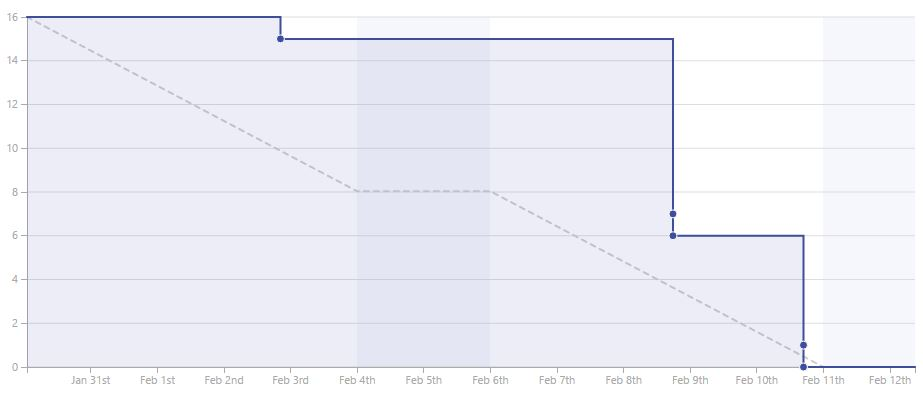
\includegraphics[width=0.99\textwidth]{sprint_0}
\caption{Burndown del \textit{sprint} 0}
\label{fig:A.1.1}
\end{figure}

\subsection{\textit{Sprint} 1}
Estas son las tareas a realizar durante esta \textit{sprint} 1:

\begin{itemize}
	\item Documentar lo realizado durante el \textit{sprint} 0.
	\item Documentar lo que se irá realizando durante este \textit{sprint} 1.
	\item Continuar probando con algoritmos de procesamiento de imágenes.
	\item Probar una aproximación con clasificadores al problema.
\end{itemize}

Puesto que en el \textit{sprint} anterior no se documentó lo realizado, durante éste se pretende documentar todo lo realizado durante el \textit{sprint} anterior y éste. Además de continuar probando con algoritmos de procesamiento de imágenes y comenzar a probar con la aproximación al problema mediante clasificadores.

En este \textit{sprint} me vi desbordado de trabajo debido a la subestimación del esfuerzo a empeñar en las distintas tareas. No siendo capaz de comenzar a probar una aproximación con clasificadores. Por ello la tarea <<Probar una aproximación con clasificadores al problema>> se vio movida al siguiente \textit{sprint}. 

A continuación, en la figura \ref{fig:A.1.2}, se muestra el diagrama \textit{burndown} de este \textit{sprint}. El cual tiene dicho aspecto debido a que muchas de las tareas se trabajaron de manera paralela, no siendo acabadas hasta el final del \textit{sprint}. Y, además, algunas de las tareas no fueron cerradas cuando se debió, aspecto que se corregirá en los siguientes \textit{sprints}.

\begin{figure}
\centering
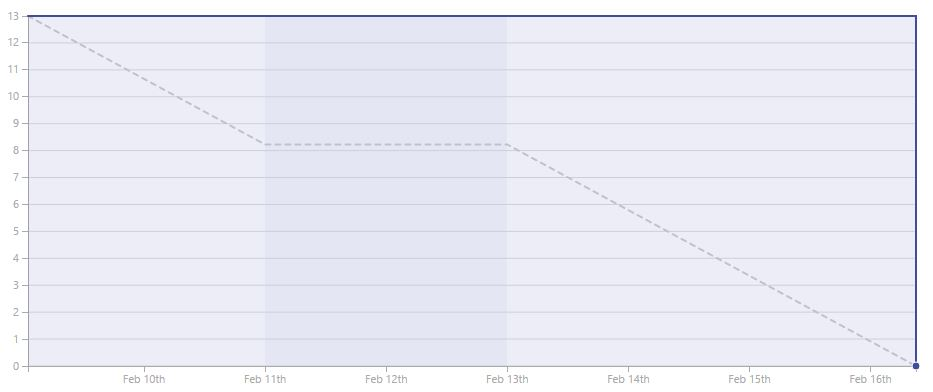
\includegraphics[width=0.99\textwidth]{sprint_1}
\caption{Burndown del \textit{sprint} 1}
\label{fig:A.1.2}
\end{figure}

\subsection{\textit{Sprint} 2}
Estas son las tareas a realizar durante este \textit{sprint} 2:

\begin{itemize}
	\item Probar una aproximación con clasificadores al problema.
	\item Aplicación del método <<Non-maximum suppression>> sobre el clasificado.
\end{itemize}

Puesto que la aproximación mediante reconocimiento de imágenes no reflejaba unos resultados muy positivos, durante la reunión mantenida con los tutores se decidió el uso de una técnica distinta. Nos referimos a la utilización  de un clasificador, junto a un descriptor visual.

Debido a que todavía no se poseían suficientes imágenes para el estudio del problema mediante esta técnica, lo que se decidió es aplicarla sobre otro problema de características similares, como es el reconocimiento de caras en imágenes. Con unos resultados bastante positivos debido a distintos razonamientos explicados en la Memoria, sección de Aspectos relevantes del proyecto.

A continuación, en la figura \ref{fig:A.1.3}, se muestra el diagrama \textit{burndown} de este \textit{sprint}.

\begin{figure}
\centering
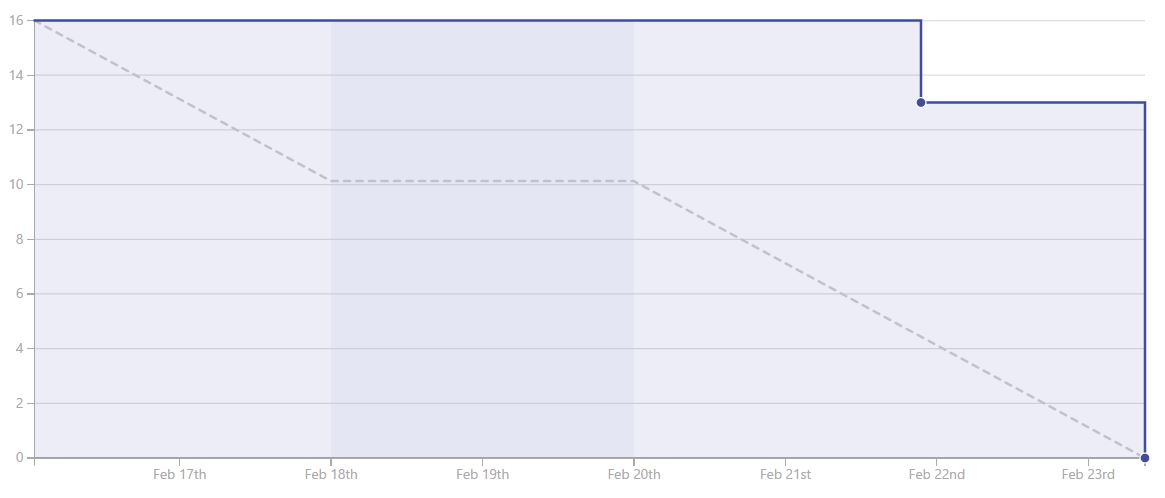
\includegraphics[width=0.99\textwidth]{sprint_2}
\caption{Burndown del \textit{sprint} 2}
\label{fig:A.1.3}
\end{figure}

\subsection{\textit{Sprint} 3}
Estas son las tareas a realizar durante este \textit{sprint} 3:

\begin{itemize}
	\item Reorganizar los \textit{Jupyter Notebooks}.
	\item Probar distintos clasificadores y métricas.
	\item Enviar fotos rotadas al clasificador.
\end{itemize}

Durante este \textit{sprint}, primero, se reorganizó la estructura del proyecto. Aportando mucho más orden y claridad a nuestro proyecto. Después, se introdujeron múltiples clasificadores y métricas, los cuales introduciré en mayor medida en la memoria, como \textit{Random Forest}~\cite{randomforest} o \textit{Gradient tree boosting}~\cite{gradientboosting}. Por último, se enviaron imágenes rotadas al clasificador, con el fin de poder analizar una posible problemática.

A continuación, en la figura \ref{fig:A.1.4}, se muestra el diagrama \textit{burndown} de este \textit{sprint}.

\begin{figure}
\centering
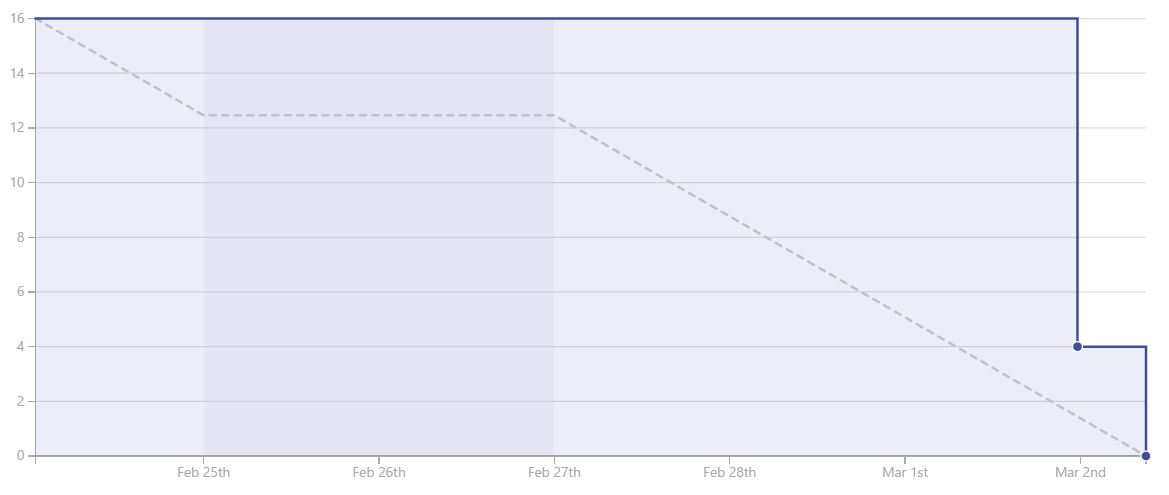
\includegraphics[width=0.99\textwidth]{sprint_3}
\caption{Burndown del \textit{sprint} 3}
\label{fig:A.1.4}
\end{figure}

\subsection{\textit{Sprint} 4}
Estas son las tareas a realizar durante este \textit{sprint} 4:

\begin{itemize}
	\item Implementación de \textit{Data Augmentation} en nuestro conjunto de entrenamiento.
	\item Implementación de controles de usuario.
\end{itemize}

Durante este \textit{sprint} se aplicó en nuestro conjunto de entrenamiento la técnica \textit{Data augmentation}. Esta técnica nos permitió aumentar el tamaño de nuestro conjunto de entrenamiento enormemente. 

Además, se realizó un \textit{notebook}\footnote{Siempre que nos referimos a un \textit{notebook}, a lo que nos referimos es a un \textit{Jupyter Notebook}}, con controles de usuario, los cuales nos permiten escoger entre clasificadores, imágenes y probabilidades. Permitiendo la continua interacción entre el usuario y la clasificación de una imagen, sin la necesidad de modificar el código por parte del usuario del notebook para cambiar entre las distintas opciones.

A continuación, en la figura \ref{fig:A.1.5}, se muestra el diagrama \textit{burndown} de este \textit{sprint}.

\begin{figure}
\centering
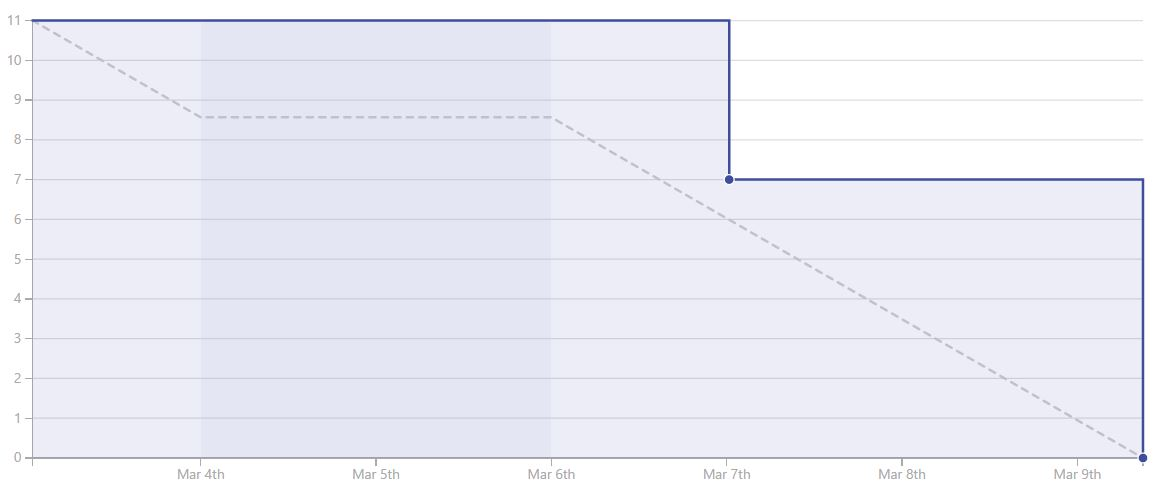
\includegraphics[width=0.99\textwidth]{sprint_4}
\caption{Burndown del \textit{sprint} 4}
\label{fig:A.1.5}
\end{figure}


\subsection{\textit{Sprint} 5}
Estas son las tareas a realizar durante este \textit{sprint} 5:

\begin{itemize}
	\item Implementar un \textit{file chooser} 
	\item Añadir más clasificadores.
	\item Correciones en la documentación.
	\item Estudiar como implementar un etiquetador de imágenes.
\end{itemize}

Durante este \textit{sprint} se añadieron los clasificadores que deseábamos, es decir, un clasificador bayesiano y un clasificador mediante regresión logística. Además, se añadió un \textit{file chooser} que nos permitiría, desde ese momento, escoger la imagen que deseemos dentro de nuestro sistema operativo. En cuanto a la documentación, se corrigió toda la  realizada hasta ese momento. Y, por último, se hizo un estudio básico sobre como implementar un etiquetador de imágenes mediante un \textit{Widget} de \textit{Python}. Aunque, esta última tarea no tuviese ningún producto resultante en este \textit{sprint}.

A continuación, en la figura \ref{fig:A.1.6}, se muestra el diagrama \textit{burndown} de este \textit{sprint}.

\begin{figure}
\centering
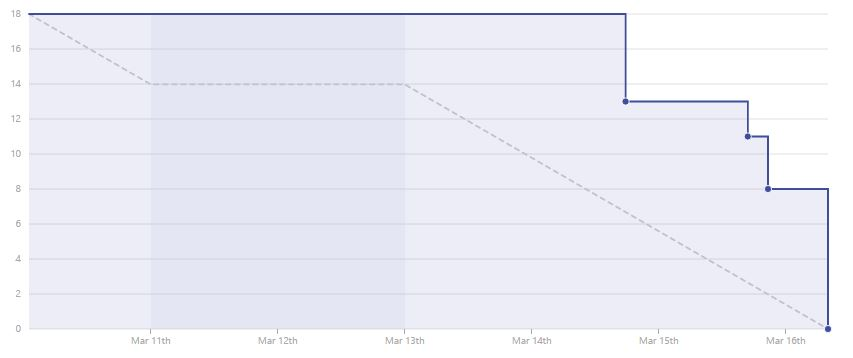
\includegraphics[width=0.99\textwidth]{sprint_5}
\caption{Burndown del \textit{sprint} 5}
\label{fig:A.1.6}
\end{figure}

\subsection{\textit{Sprint} 6}
Estas son las tareas a realizar durante este \textit{sprint} 6:

\begin{itemize}
	\item Estudiar los \textit{Widgets} personalizados de \textit{Jupyter Notebook} e \textit{Ipython}.
\end{itemize}

Aunque este \textit{sprint} se encuentre compuesto por una única tarea, no era menos complejo por ello. El objetivo de este \textit{sprint} era obtener un \textit{Widget} capaz de etiquetar imágenes. Pero en la realización de este se encontraron multiples problemas. Obteniendo como producto resultante tres posibles alternativas con aspectos a corregir.

Por lo tanto, en la figura \ref{fig:A.1.7} mostramos el diagrama \textit{burndown}, poco esclarecedor, de este \textit{sprint}.

\begin{figure}
\centering
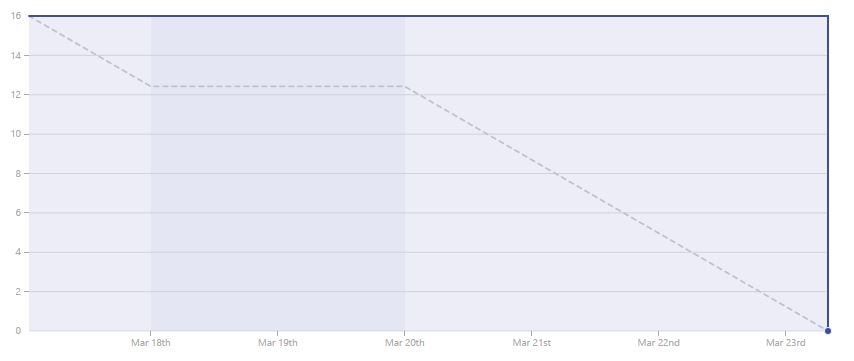
\includegraphics[width=0.99\textwidth]{sprint_6}
\caption{Burndown del \textit{sprint} 6}
\label{fig:A.1.7}
\end{figure}



\subsection{\textit{Sprint} 7}
Estas son las tareas a realizar durante este \textit{sprint} 7:

\begin{itemize}
	\item Estudiar \textit{Bag of Words}.
	\item Añadir mayor parametrización al \textit{Jupyter Notebook UI}.
	\item Corregir \textit{bugs} del Widget previamente implementado.
\end{itemize}

Durante este \textit{sprint} se consiguió, en primer lugar, corregir una de las alternativas del etiquetador de imágenes, o \textit{Widget}, desarrolladas durante el \textit{sprint} anterior. Además, se corrigieron y añadieron múltiples parámetros en el \textit{Jupyter Notebook UI} y en las clases utilizadas por este \textit{Notebook}. Y, por ultimo, se realizo un estudio sobre un modelo ampliamente usado para tareas de clasificación, llamado \textit{Bag of Words}.

A continuación, en la figura \ref{fig:A.1.8}, se muestra el diagrama \textit{burndown} de este \textit{sprint}.

\begin{figure}
\centering
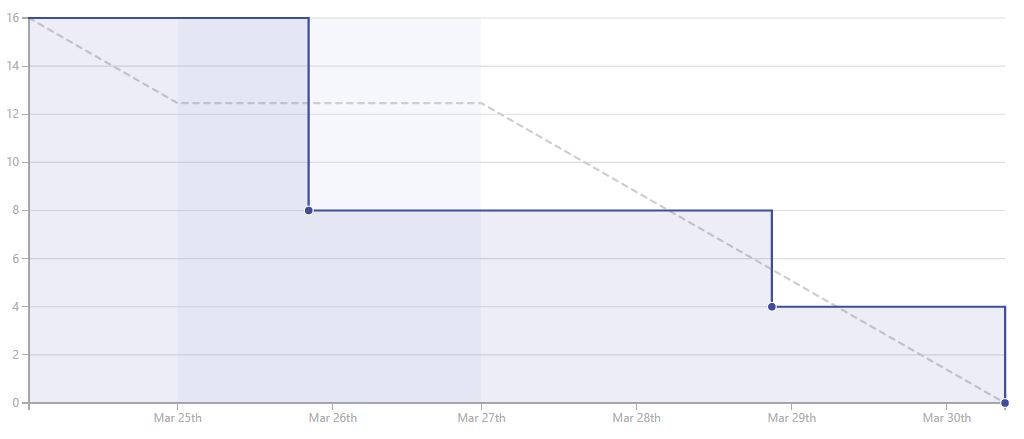
\includegraphics[width=0.99\textwidth]{sprint_7}
\caption{Burndown del \textit{sprint} 7}
\label{fig:A.1.8}
\end{figure}


\subsection{\textit{Sprint} 8}
Estas son las tareas a realizar durante este \textit{sprint} 8:

\begin{itemize}
	\item Implementar la funcionalidad de obtención de imágenes en el etiquetador de imágenes, o \textit{Widget}.
	\item Mejorar la interfaz del etiquetador de imágenes.
	\item Crear un primer prototipo de interfaz de usuario.
\end{itemize}

Durante este \textit{sprint} se realizó un primer prototipo de interfaz de  usuario. Partiendo de este prototipo, se mejoró la interfaz del etiquetador de imágenes. Consiguiendo, así, una interfaz adecuada para el cliente. Además, se implemento la funcionalidad que nos permitiría obtener una imágen resultante de cada etiqueta realizada en las distintas imágenes.

A continuación, en la figura \ref{fig:A.1.9}, se muestra el diagrama \textit{burndown} de este \textit{sprint}.

\begin{figure}
\centering
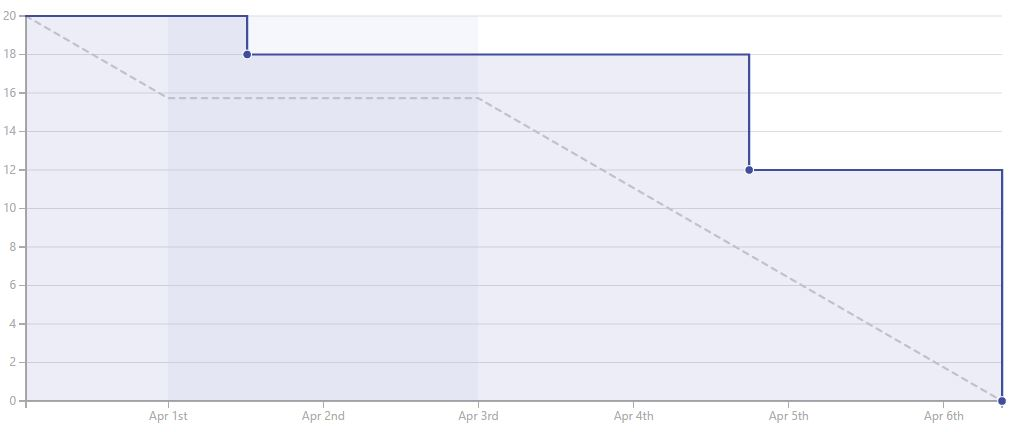
\includegraphics[width=0.99\textwidth]{sprint_8}
\caption{Burndown del \textit{sprint} 8}
\label{fig:A.1.9}
\end{figure}

\subsection{\textit{Sprint} 9}

Este \textit{sprint} tendrá una duración de dos semanas. Debido  a la carga de trabajo asociada a este \textit{sprint} y al ser días no lectivos por las vacaciones de Semana Santa. 

Estas son las tareas a realizar durante este \textit{sprint} 9:

\begin{itemize}
	\item Añadir un texto a cada etiqueta que realizamos en una imagen.
	\item Añadir notificaciones al usuario en la carga y guardado de imágenes.
	\item Guardar las coordenadas de las etiquetas de cada imagen.
	\item Cargar las etiquetas de una imagen que haya sido previamente etiquetada.
	\item Controlar que el usuario no cree etiquetas en el SVG pero fuera de la imagen.
	\item Añadir la posibilidad de eliminar etiquetas previamente realizadas.
	\item Añadir un botón que permita guardar imágenes como negativos.
	\item Corregir los \textit{notebooks} creados para la técnica \textit{Bag of Words}.
\end{itemize}

Durante este \textit{sprint} se completaron todas las tareas asignadas, excepto la corrección de los \textit{notebooks} para la técnica \textit{Bag of Words}. Los cuales no se revisaron porque no se utilizarían por el momento.

A continuación, en la figura \ref{fig:A.1.10}, se muestra el diagrama \textit{burndown} de este \textit{sprint}.

\begin{figure}
\centering
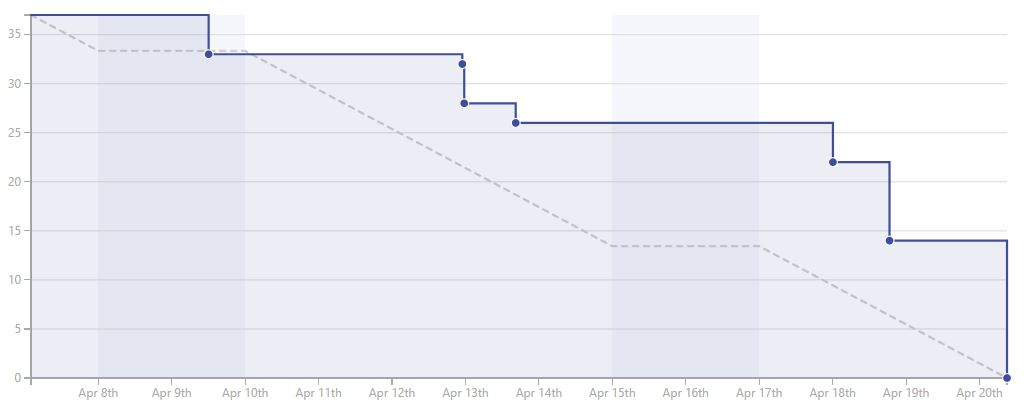
\includegraphics[width=0.99\textwidth]{sprint_9}
\caption{Burndown del \textit{sprint} 9}
\label{fig:A.1.10}
\end{figure}


\subsection{\textit{Sprint} 10}

Estas son las tareas a realizar durante este \textit{sprint} 10:

\begin{itemize}
	\item Tratar de reentrenar a \textit{YOLO}.
	\item Corregir errores en la carga de etiquetas.
	\item Mejorar la interfaz del etiquetador de imágenes.
	\item Documentación: manual de usuario del etiquetador de imágenes.
	\item Documentación: diseño(prototipo).
\end{itemize}

Durante este \textit{sprint} se comenzaron las pruebas con el detector automático de objetos, para su futura adaptación a la detección de fitolitos. Además, se trataron de solucionar algunos errores presentes en el etiquetador. Y, finalmente, se documentó en la medida de lo posible el manual del etiquetador. Tratando de facilitar su uso por parte de los usuarios, en breves momentos.

A continuación, en la figura \ref{fig:A.1.11}, se muestra el diagrama \textit{burndown} de este \textit{sprint}.

\begin{figure}
\centering
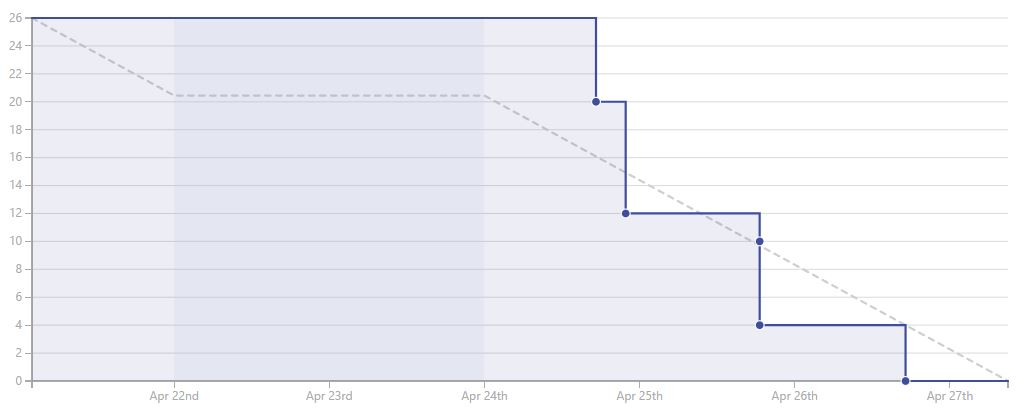
\includegraphics[width=0.99\textwidth]{sprint_10}
\caption{Burndown del \textit{sprint} 10}
\label{fig:A.1.11}
\end{figure}

\subsection{\textit{Sprint} 11}

Estas son las tareas a realizar durante este \textit{sprint} 11:

\begin{itemize}
	\item Documentación: aspectos relevantes
	\item Documentación: conceptos \textit{YOLO} y \textit{BoW}
	\item Documentación: técnicas y herramientas.
	\item Documentación: manual del programador.
	\item Poner correctamente los separadores de archivo en Linux Y Windows.
	\item Crear script para la lectura de las coordenadas desde \textit{YOLO}.
	\item Documentación: \textit{README}.
\end{itemize}

Durante este \textit{sprint}, principalmente, se trato de documentar algunos de los aspectos de la memoria. Y, por último, se creó un \textit{script} para la lectura y conversión de las coordenadas para el entrenamiento de \textit{YOLO}.

A continuación, en la figura \ref{fig:A.1.12}, se muestra el diagrama \textit{burndown} de este \textit{sprint}.

\begin{figure}
\centering
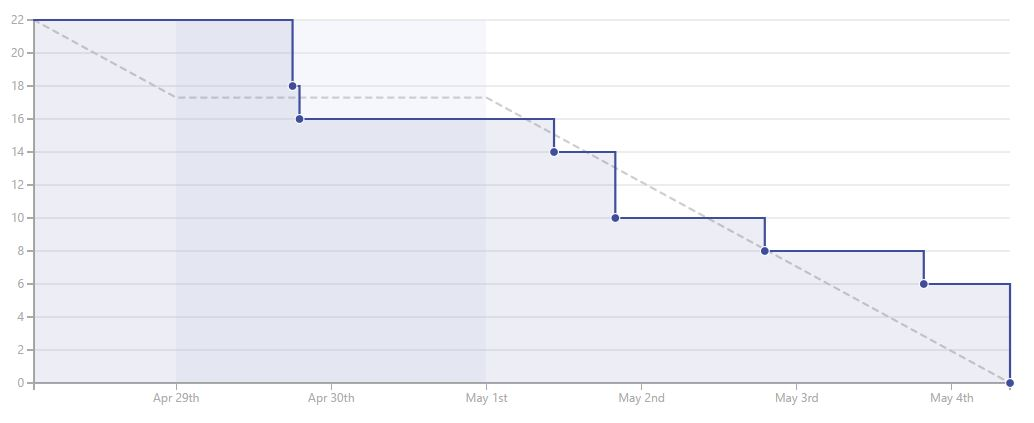
\includegraphics[width=0.99\textwidth]{sprint_11}
\caption{Burndown del \textit{sprint} 11}
\label{fig:A.1.12}
\end{figure}

\subsection{\textit{Sprint} 12}

Estas son las tareas a realizar durante este \textit{sprint} 12:

\begin{itemize}
	\item \textit{Data augmentation}: rotar imágenes y coordenadas en ángulos de 90 grados.
	\item \textit{Data augmentation}: espejar imágenes.
	\item \textit{Data augmentation}: aplicar ruidos a las imágenes.
	\item \textit{Data augmentation}: realizar cambios de tamaño en las imágenes.
	\item Documentación: introducción.
	\item Documentación: objetivos del proyecto.
	\item Documentación: trabajos relacionados.
	\item Documentación: Documentación: diseño arquitectónico y procedimental.
\end{itemize}

Durante este \textit{sprint} se trato de continuar escribiendo algunos de los aspectos todavía no documentados hasta el momento. Y se creo una herramienta para la aplicación de técnicas de \textit{data augmentation} sobre un conjunto de imágenes. Además, la última de las tareas planteadas para este \textit{sprint} fue completada en un sprint más adelante por ser muy subestimada en cuanto al esfuerzo requerido.

A continuación, en la figura \ref{fig:A.1.13}, se muestra el diagrama \textit{burndown} de este \textit{sprint}.

\begin{figure}
\centering
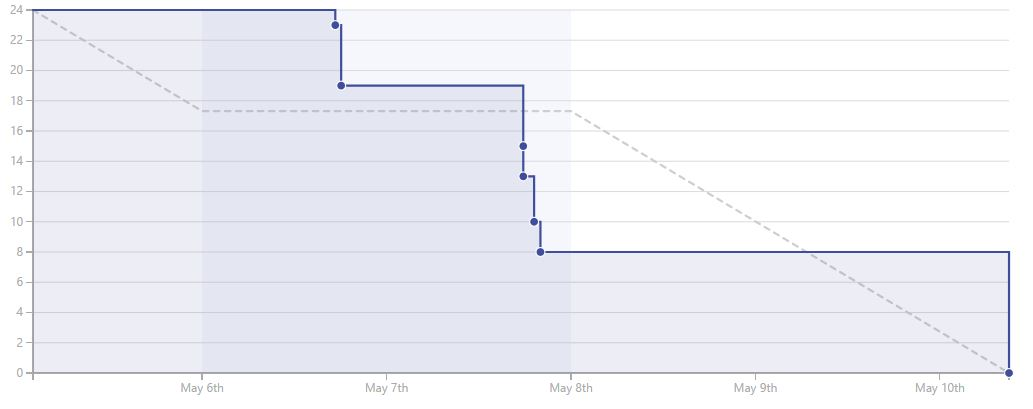
\includegraphics[width=0.99\textwidth]{sprint_12}
\caption{Burndown del \textit{sprint} 12}
\label{fig:A.1.13}
\end{figure}

\subsection{\textit{Sprint} 13}

Estas son las tareas a realizar durante este \textit{sprint} 13:

\begin{itemize}
	\item \textit{Data augmentation}: generador de imágenes.
	\item \textit{Data augmentation}: aplicar filtros en las imágenes (clarecer,oscurecer).
	\item Entrenar por primera vez a YOLO con un primer dataset de fitolitos.
\end{itemize}

Durante este \textit{sprint} se finalizo el generador de imágenes que aplicaba las técnicas de \textit{data augmentation}, implementadas durante el \textit{sprint} anterior, para generar un conjunto de imágenes mucho mayor. Y, además, dado que nuestros clientes nos enviaron un conjunto de imágenes etiquetadas de fitolitos, comenzamos con los primeros entrenamientos a \textit{YOLO}.

A continuación, en la figura \ref{fig:A.1.14}, se muestra el diagrama \textit{burndown} de este \textit{sprint}.

\begin{figure}
\centering
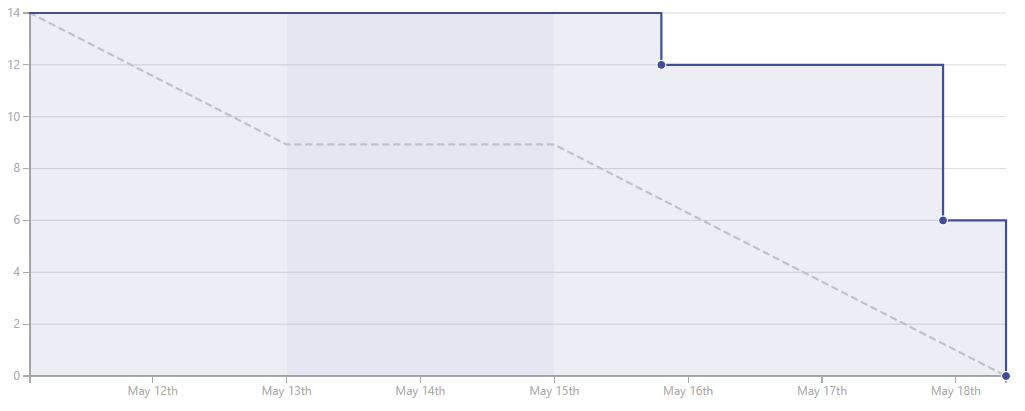
\includegraphics[width=0.99\textwidth]{sprint_13}
\caption{Burndown del \textit{sprint} 13}
\label{fig:A.1.14}
\end{figure}

\subsection{\textit{Sprint} 14}

Estas son las tareas a realizar durante este \textit{sprint} 14:

\begin{itemize}
	\item Correcciones menores en fichero \textit{README}.
	\item Evaluar los resultados de \textit{YOLO} con un primer dataset.
	\item Entrenar a YOLO con el dataset aplicando \textit{data augmentation}.
\end{itemize}

Durante este \textit{sprint} se entrenó a YOLO, con un dataset de un tamaño mayor. Además, se completaron otras tareas pendientes de las semanas anteriores, relativas a la documentación y a la evaluación del modelo generado por el entrenamiento.

A continuación, en la figura \ref{fig:A.1.15}, se muestra el diagrama \textit{burndown} de este \textit{sprint}.

\begin{figure}
\centering
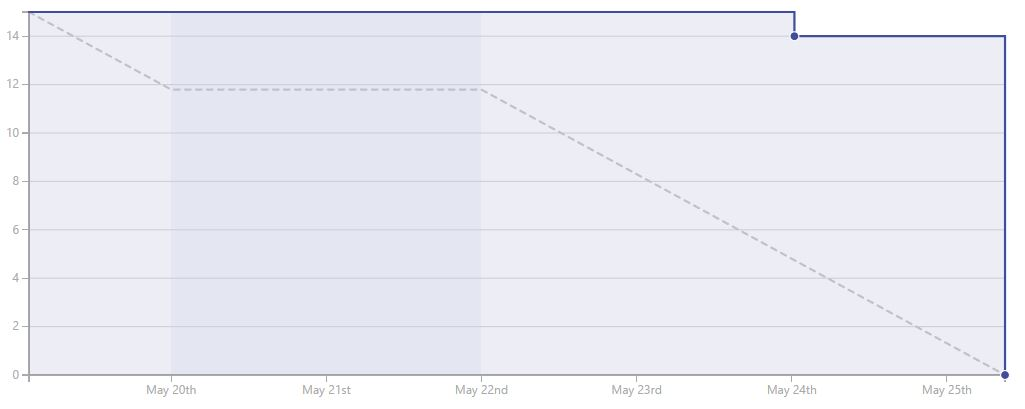
\includegraphics[width=0.99\textwidth]{sprint_14}
\caption{Burndown del \textit{sprint} 14}
\label{fig:A.1.15}
\end{figure}

\subsection{\textit{Sprint} 15}

Estas son las tareas a realizar durante este \textit{sprint} 15:

\begin{itemize}
	\item Documentación: lineas futuras.
	\item Reetiquetar un único tipo de fitolitos.
	\item Documentación: completar el anexo de planificación del proyecto.
	\item Documentación: completar los aspectos restantes del anexo de diseño.
	\item Documentación: Preparar el anexo de requisitos.
	\item Entrenar el clasificador con los fitolitos reetiquetados.
\end{itemize}

Durante esta semana, principalmente, se trato de continuar con aspectos de documentación. Y, a su vez, se continuo entrenando a \textit{YOLO} con el fin de conseguir algún resultado. 

A continuación, en la figura \ref{fig:A.1.16}, se muestra el diagrama \textit{burndown} de este \textit{sprint}.

\begin{figure}
\centering
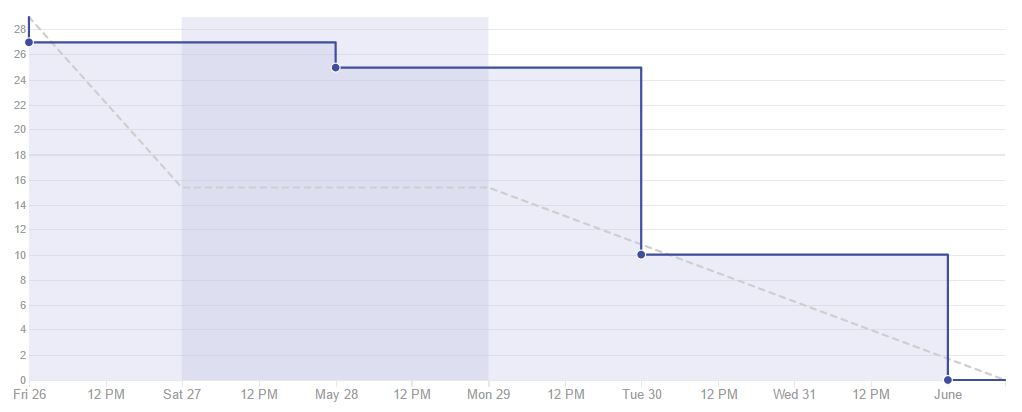
\includegraphics[width=0.99\textwidth]{sprint_15}
\caption{Burndown del \textit{sprint} 15}
\label{fig:A.1.16}
\end{figure}

\subsection{\textit{Sprint} 16}

Estas son las tareas a realizar durante este \textit{sprint} 16:

\begin{itemize}
	\item Documentación: Complejidad de la tarea.
	\item Unificar separadores en todos los fuentes.
	\item Documentación: conceptos teóricos restantes.
	\item Desarrollar teses para los distintos módulos.
\end{itemize}

Durante esta semana se unificaron los separadores del sistemas operativo, se documento y se realizaron teses para los módulos más relevantes del sistema.

A continuación, en la figura \ref{fig:A.1.17}, se muestra el diagrama \textit{burndown} de este \textit{sprint}.

\begin{figure}
\centering
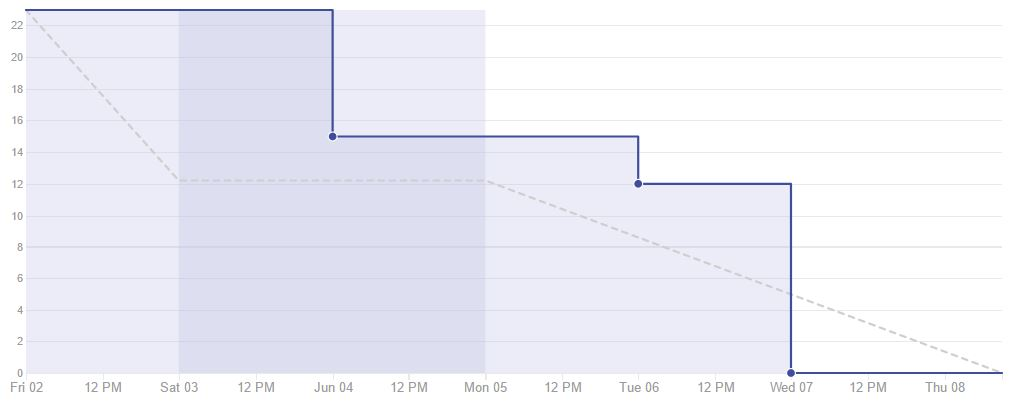
\includegraphics[width=0.99\textwidth]{sprint_16}
\caption{Burndown del \textit{sprint} 16}
\label{fig:A.1.17}
\end{figure}

\subsection{\textit{Sprint} 17}

Estas son las tareas a realizar durante este \textit{sprint} 17:

\begin{itemize}
	\item Añadir la funcionalidad de clasificar fitolitos.
\end{itemize}

Durante esta semana se volvió al enfoque mediante clasificadores. Principalmente, se trato de encontrar las distintas opciones para la clasificación de fitolitos y evaluar los resultados. Para, más tarde, aplicarlo a la detección de estos mediante ventana deslizante.

A continuación, en la figura \ref{fig:A.1.18}, se muestra el diagrama \textit{burndown} de este \textit{sprint}.

\begin{figure}
\centering
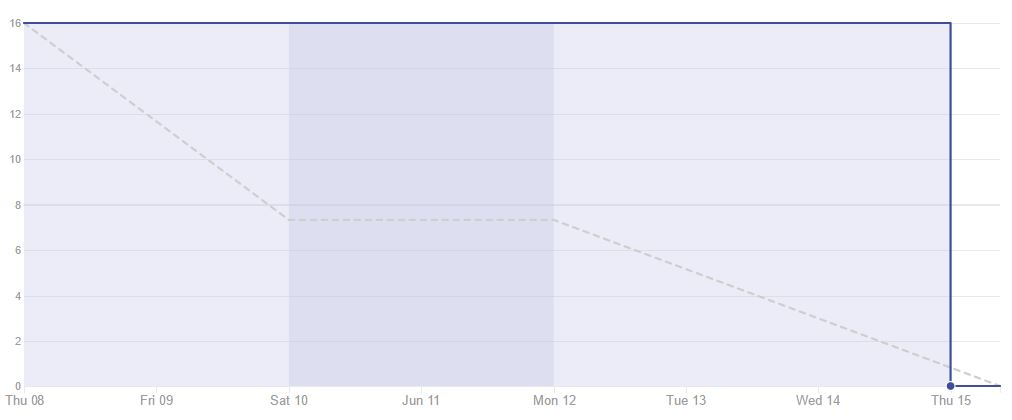
\includegraphics[width=0.99\textwidth]{sprint_17}
\caption{Burndown del \textit{sprint} 17}
\label{fig:A.1.18}
\end{figure}

\subsection{\textit{Sprint} 18}

Estas son las tareas a realizar durante este \textit{sprint} 18:

\begin{itemize}
	\item Hallar el mejor clasificador posible.
	\item Aplicar la ventana deslizante a las imágenes de fitolitos.
\end{itemize}

Durante esta semana se obtuvo el clasificador que mejor se adaptaba a la problemática mediante un \textit{script} que evaluaba las distintas opciones. Y, finalmente, se aplico a la detección de fitolitos en imágenes.

A continuación, en la figura \ref{fig:A.1.19}, se muestra el diagrama \textit{burndown} de este \textit{sprint}.

\begin{figure}
\centering
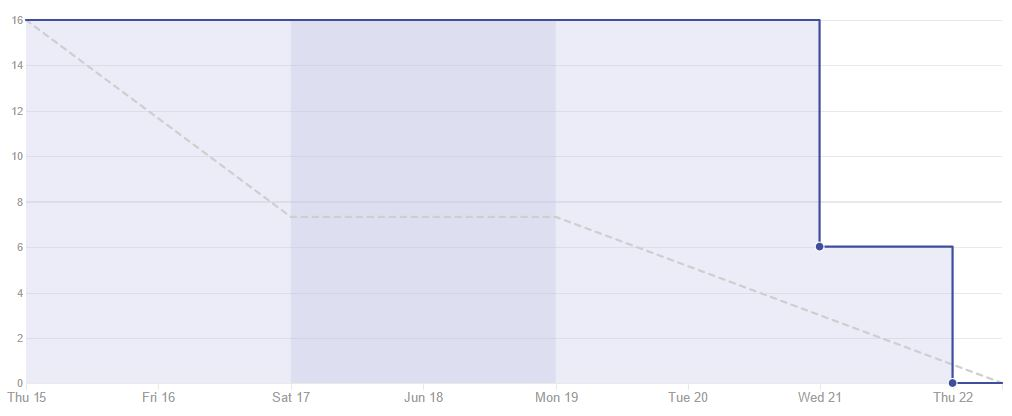
\includegraphics[width=0.99\textwidth]{sprint_18}
\caption{Burndown del \textit{sprint} 18}
\label{fig:A.1.19}
\end{figure}

\section{Estudio de viabilidad}

\subsection{Viabilidad económica}
En esta sección se realiza un análisis de los costes económicos que hubiera supuesto el desarrollo de este proyecto en un entorno empresarial.

\subsubsection{Coste del personal}
Este proyecto ha sido desarrollado por un único desarrollador a tiempo parcial. En la tabla \ref{tabla:costespersonales} muestro el desglose de los costes ocasionados por el salario que hubiese recibido en una situación real.

\tablaSmallSinColores{Costes de personal}{p{4.5cm} p{.25cm} p{2.5cm}}{costespersonales}{
  \multicolumn{3}{p{6cm}}{\textbf{Costes de personal}} \\
 }
 {
  Salario mensual neto  & 1500\euro{} \\
  Retención IRPF (15\%) & \euro{} \\
  Seguridad social (29,9\%) & \euro{} \\
  Salario mensual bruto  & \euro{} \\\hline
  Salario total(4 meses)  & \euro{} \\
  }

\subsubsection{Coste del \textit{software} y \textit{hardware}}



\subsubsection{Costes totales}



\subsection{Viabilidad legal}

En este apartado enuncio las distintas librerías utilizadas junto a sus licencias, en todos sus casos de código abierto. Véase la tabla \ref{tabla:licencias}. Si se desea indagar más sobre las distintas librerías se recomienda ver la sección de herramientas y técnicas dentro de la memoria.
 
  \begin{table}
  \begin{center}
   \begin{tabular}{p{3.5cm} p{1.5cm} p{2.5cm}}
    \toprule
    \textbf{Librería} & \textbf{Versión} & \textbf{Licencia} \\
    \otoprule
    Numpy & 1.12 & BSD \\
    scikit-learn & 0.18 & BSD \\
    scikit-image & 0.13 & BSD \\
    Matplotlib & 1.12 & PSF \\
    Jupyter Notebook & 1 & BSD \\
    Jupyter Dashboards & 0.6 & BSD \\
	Ipython File Upload & 0.1.2 & MIT \\
	darkflow & 0 & GPL 3 \\
    \bottomrule
   \end{tabular}
   \caption{Licencias de las librerías}
   \label{tabla:licencias}
  \end{center}
 \end{table}
 
 Finalmente, este proyecto esta publicado bajo la licencia \textit{BSD 3-clause} con la que se permite un libre uso, modificación, distribución y uso privado de este. Sin embargo, con la condición de que el código debe ser suministrado en todas las ocasiones junto a la licencia que expone las distintas garantías de uso. Para finalizar, esta licencia introduce una muy limitada responsabilidad sobre la utilización de este proyecto y ningún tipo de garantía.

\apendice{Especificación de Requisitos}

\section{Introducción}
En este anexo se pretenden indicar los distintos objetivos propuestos en el desarrollo de este proyecto. Así, como el conjunto de requisitos y sus especificaciones.

\section{Objetivos generales}
Los objetivos generales de este proyecto son los siguientes:

\begin{itemize}
	\item Crear un sistema capaz de reconocer fitolitos automáticamente en una imagen.
	\item Crear un sistema de etiquetación de fitolitos. Con el que podamos crear un conjunto de imágenes etiquetadas para llevar a cabo el sistema automático de reconocimiento de fitolitos.
	\item Crear un sistema que nos permita multiplicar en cantidad nuestro conjunto de imágenes. Debido al diminuto conjunto de imágenes que nos ha sido proporcionado.
\end{itemize}

\section{Catalogo de requisitos}
Derivados de los objetivos anteriores, poseemos un conjunto de requisitos para el conjunto de aplicaciones resultantes de este proyecto.

\begin{itemize}
	\item \textbf{RF-1} Crear un sistema capaz de reconocer fitolitos automáticamente.
	\begin{itemize}
		\item \textbf{RF-1.1} Subir una nueva imagen y predecir donde se encuentran los distintos fitolitos.	\end{itemize}
	\item \textbf{RF-2} Crear una aplicación que permita el etiquetado de fitolitos. Con las siguientes funcionalidades:
	\begin{itemize}
		\item \textbf{RF-2.1} Escoger una imagen dentro de nuestro sistema operativo.
		\item \textbf{RF-2.2} Elegir entre los distintos tipos de fitolitos.
		\item \textbf{RF-2.3} Eliminar etiquetas realizadas sobre una imagen.
		\item \textbf{RF-2.5} Cargar una imagen previamente etiquetada junto a sus etiquetas.
		\item \textbf{RF-2.6} Guardar las coordenadas de las etiquetas y las imágenes de manera persistente.
		\item \textbf{RF-2.7} Notificar al usuario de los distintos eventos.
		\item \textbf{RF-2.8} Mostrar el tipo de fitolito etiquetado encima de cada etiqueta.
	\end{itemize}
	\item \textbf{RF-3} Crear una herramienta capaz de multiplicar el conjunto de imágenes etiquetadas de fitolitos mediante la aplicación de técnicas de \textit{data augmentation}.
	\begin{itemize}
		\item \textbf{RF-3.1} Elegir el número de imágenes resultantes.
		\item \textbf{RF-3.2} Reescalarlas.		
		\item \textbf{RF-3.3} Rotarlas.
		\item \textbf{RF-3.4} Espejarlas.
		\item \textbf{RF-3.5} Aplicarlas ruidos.
		\item \textbf{RF-3.6} Aplicarlas filtros de oscurecimiento y aclaramiento.
		\item \textbf{RF-3.7} Aplicarlas aleatoriamente las distintas modificaciones anteriores, permitiendo el mayor número de combinaciones posible.
	\end{itemize}
\end{itemize}


\section{Especificación de requisitos}

\subsection{Diagramas de casos de uso}

\begin{figure}
\centering
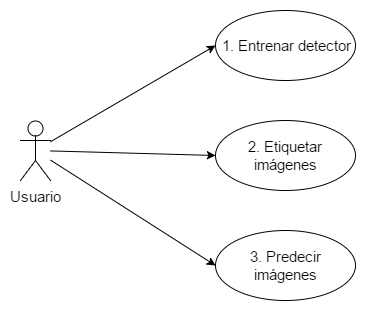
\includegraphics[width=0.5\textwidth]{dia_uc}
\caption{Diagrama general de casos de uso}
\label{fig:C.B.1}
\end{figure}

\begin{figure}
\centering
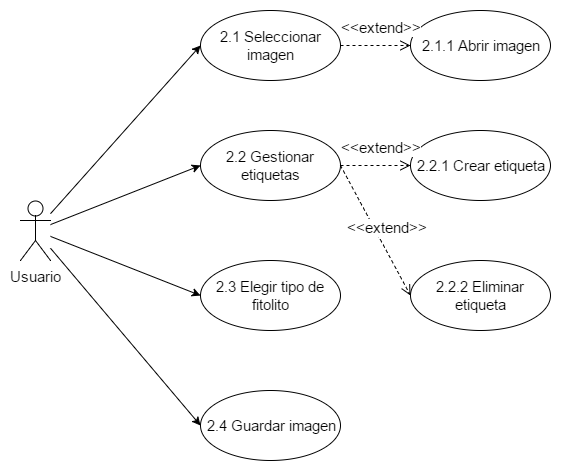
\includegraphics[width=0.9\textwidth]{dia_uc1}
\caption{Diagrama extendido de casos de uso}
\label{fig:C.B.1}
\end{figure}




\tablaSmallSinColores{Caso de uso 1: Entrenar detector}{p{3cm} p{.75cm} p{9.5cm}}{tablaUC1}{
  \multicolumn{3}{l}{Caso de uso 1:  Entrenar detector} \\
 }
 {
  Descripción                            & \multicolumn{2}{p{10.25cm}}{Permite al usuario entrenar el detector automático de fitolitos.} \\\hline
  \multirow{2}{3.5cm}{Requisitos}  & \multicolumn{2}{p{10.25cm}}{RF-1} 
  \\\cline{2-3}
                                         & \multicolumn{2}{p{10.25cm}}{RF-1.1}
                                         \\\hline
  Precondiciones                         &  \multicolumn{2}{p{10.25cm}}{Tener instalado \textit{darkflow}.}   \\\hline
  \multirow{2}{3.5cm}{Secuencia normal}  & Paso & Acción \\\cline{2-3}
                                         & 1    & El usuario lanza el comando de entrenamiento.
  \\\cline{2-3}
                                         & 2    & Se carga el modelo.
  \\\cline{2-3}
                                         & 3    & Se cargan los pesos del modelo.
    \\\cline{2-3}
                                         & 4    & Se convierten las coordenadas de las etiquetas.                                           	\\\cline{2-3}
                                         & 5    & Se comienza el entrenamiento. 
                                         \\\hline
  Postcondiciones                        & \multicolumn{2}{p{10.25cm}}{Se guardan unos ficheros con los pesos resultantes del entrenamiento.} \\\hline
  Excepciones                        & \multicolumn{2}{p{10.25cm}}{La elección de opciones no compatibles entre sí.}\\\hline
  Importancia                            & Alta \\\hline
  Urgencia                               & Media \\
}





\tablaSmallSinColores{Caso de uso 2: Etiquetar imágenes}{p{3cm} p{.75cm} p{9.5cm}}{tablaUC2}{
  \multicolumn{3}{l}{Caso de uso 2:  Etiquetar imágenes} \\
 }
 {
  Descripción                            & \multicolumn{2}{p{10.25cm}}{Permite al usuario identificar los múltiples tipos de fitolitos.} \\\hline
  \multirow{2}{3.5cm}{Requisitos}  &\multicolumn{2}{p{10.25cm}}{RF-2} \\\cline{2-3}
                                         & \multicolumn{2}{p{10.25cm}}{RF-2.1} \\\cline{2-3}
                                         & \multicolumn{2}{p{10.25cm}}{RF-2.2}  \\\cline{2-3}
                                         & \multicolumn{2}{p{10.25cm}}{RF-2.3}  \\\cline{2-3}
                                         & \multicolumn{2}{p{10.25cm}}{RF-2.4}  \\\cline{2-3}
                                         & \multicolumn{2}{p{10.25cm}}{RF-2.5}  \\\cline{2-3}
                                         & \multicolumn{2}{p{10.25cm}}{RF-2.6}  \\\cline{2-3}
                                         & \multicolumn{2}{p{10.25cm}}{RF-2.7}  \\\cline{2-3}
                                         & \multicolumn{2}{p{10.25cm}}{RF-2.8}
                                         \\\hline
  Precondiciones                         &    \multicolumn{2}{p{10.25cm}}{Ejecutar el \textit{Jupyter Notebook}.}    \\\hline
  \multirow{2}{3.5cm}{Secuencia normal}  & Paso & Acción \\\cline{2-3}
                                         & 1    & El usuario selecciona una imagen.
  \\\cline{2-3}
                                         & 2    & La imagen se carga.
  \\\cline{2-3}
                                         & 3    & El usuario etiqueta los fitolitos.
    \\\cline{2-3}
                                         & 4    & El usuario pulsa en el botón guardar.                                           	\\\cline{2-3}
                                         & 5    & Se guardan las imágenes y coordenadas. 
                                         \\\hline
  Postcondiciones                        & \multicolumn{2}{p{10.25cm}}{Se guardan los ficheros que almacenan las coordenadas de las etiquetas y las imágenes.} \\\hline
  Excepciones                        & \multicolumn{2}{p{10.25cm}}{Tratar de cargar un documento distinto a una imagen.}\\\hline
  Importancia                            & Alta \\\hline
  Urgencia                               & Alta \\
}




\tablaSmallSinColores{Caso de uso 3: Predecir imágenes}{p{3cm} p{.75cm} p{9.5cm}}{tablaUC3}{
  \multicolumn{3}{l}{Caso de uso 3:  Predecir imágenes} \\
 }
 {
  Descripción                            & \multicolumn{2}{p{10.25cm}}{Permite al usuario identificar los fitolitos en una imagen.} \\\hline
  \multirow{2}{3.5cm}{Requisitos}  &\multicolumn{2}{p{10.25cm}}{RF-1} \\\cline{2-3}
                                         & \multicolumn{2}{p{10.25cm}}{RF-1.1} \\\hline
  Precondiciones                         &    \multicolumn{2}{p{10.25cm}}{Tener instalado \textit{darkflow}.}    \\\hline
  \multirow{2}{3.5cm}{Secuencia normal}  & Paso & Acción \\\cline{2-3}
                                         & 1    & El usuario escoge una imagen.
  \\\cline{2-3}
                                         & 2    & El usuario lanza el comando o script que predice una imagen.
  \\\cline{2-3}
                                         & 3    & Se carga el modelo.
    \\\cline{2-3}
                                         & 4    & Se cargan los pesos del modelo.                                           	\\\cline{2-3}
                                         & 5    & Se predice la imagen. 
    \\\cline{2-3}
                                         & 6    & Se muestran los resultados. 
                                         \\\hline
  Postcondiciones                        & \multicolumn{2}{p{10.25cm}}{} \\\hline
  Excepciones                        & \multicolumn{2}{p{10.25cm}}{Tratar de cargar un documento distinto a una imagen.
  Escoger erróneamente las configuraciones.}\\\hline
  Importancia                            & Alta \\\hline
  Urgencia                               & Alta \\
}




\tablaSmallSinColores{Caso de uso 2.1: Seleccionar imagen}{p{3cm} p{.75cm} p{9.5cm}}{tablaUC1.1}{
  \multicolumn{3}{l}{Caso de uso 2.1:  Seleccionar imagen} \\
 }
 {
  Descripción                            & \multicolumn{2}{p{10.25cm}}{El usuario puede seleccionar una imagen desde su sistema operativo. La cual se carga, muestra y finalmente se le permite etiquetarla.} \\\hline
  \multirow{2}{3.5cm}{Requisitos}  &\multicolumn{2}{p{10.25cm}}{RF-2} \\\cline{2-3}
                                         & \multicolumn{2}{p{10.25cm}}{RF-2.1} \\\cline{2-3}
                                         & \multicolumn{2}{p{10.25cm}}{RF-2.5}  \\\cline{2-3}
                                         & \multicolumn{2}{p{10.25cm}}{RF-2.7}  \\\cline{2-3}
                                         & \multicolumn{2}{p{10.25cm}}{RF-2.8}
                                         \\\hline
  Precondiciones                         &   Ninguna   & 
  \\\hline
  \multirow{2}{3.5cm}{Secuencia normal}  & Paso & Acción \\\cline{2-3}
                                         & 1    & El usuario pulsa el botón de subida de imágenes. 
  \\\cline{2-3}
                                         & 2    & El usuario selecciona una imagen.
  \\\cline{2-3}
                                         & 3    & El usuario pulsa el botón de abrir imagen.
    \\\cline{2-3}
                                         & 4    & Se carga la nueva imagen.                                           	\\\cline{2-3}
                                         & 5    & Se notifica al usuario. 
                                         \\\hline
  Postcondiciones                        & \multicolumn{2}{p{10.25cm}}{La imagen se muestra por pantalla.} \\\hline
  Excepciones                        & \multicolumn{2}{p{10.25cm}}{No se ha seleccionado una imagen, sino un documento u otro tipo de fichero.}\\\hline
  Importancia                            & Alta \\\hline
  Urgencia                               & Alta \\\hline
  Comentarios                            & & \\
}




\tablaSmallSinColores{Caso de uso 2.2: Gestionar etiquetas}{p{3cm} p{.75cm} p{9.5cm}}{tablaUC2.2.2}{
  \multicolumn{3}{l}{Caso de uso 2.2:  Gestionar etiquetas} \\
 }
 {
  Descripción                            & \multicolumn{2}{p{10.25cm}}{El usuario podrá crear y eliminar etiquetas.} \\\hline
  \multirow{2}{3.5cm}{Requisitos}  & \multicolumn{2}{p{10.25cm}}{RF-2}  \\\cline{2-3}  & \multicolumn{2}{p{10.25cm}}{RF-2.3}  \\\cline{2-3}  & \multicolumn{2}{p{10.25cm}}{RF-2.8}  \\\hline
  Precondiciones                         &   Ninguna   & \\\hline
  \multirow{2}{3.5cm}{Secuencia normal}  & Paso & Acción \\\cline{2-3}
                                         & 1    & Si el usuario clica sobre una <<x>>. 
  \\\cline{2-3}
                                         & 1.2    & Se borra etiqueta.  
  \\\cline{2-3}
                                         & 2    & Sino:
  \\\cline{2-3}
                                         & 2.2    & Se crea una etiqueta.  \\\hline
  Postcondiciones                        & \multicolumn{2}{p{10.25cm}}{ Se cambia el estado de las etiquetas.} \\\hline
  Excepciones                        & \multicolumn{2}{p{10.25cm}}{Ninguna.}\\\hline
  Importancia                            & Alta \\\hline
  Urgencia                               & Alta \\\hline
  Comentarios                            & \multicolumn{2}{p{10.25cm}}{Se permite crear etiquetas fuera de la imagen y sin haber cargado una imagen. Pero estas no se guardarán.} \\
}





\tablaSmallSinColores{Caso de uso 2.3: Elegir tipo de fitolito}{p{3cm} p{.75cm} p{9.5cm}}{tablaUC2.3}{
  \multicolumn{3}{l}{Caso de uso 2.3:  Elegir tipo de fitolito} \\
 }
 {
  Descripción                            & \multicolumn{2}{p{10.25cm}}{El usuario puede elegir entre los distintos tipos de fitolito antes de realizar una etiqueta.} \\\hline
  \multirow{2}{3.5cm}{Requisitos}  & \multicolumn{2}{p{10.25cm}}{RF-2} \\\cline{2-3}  & \multicolumn{2}{p{10.25cm}}{RF-2.2}  \\\cline{2-3}  & \multicolumn{2}{p{10.25cm}}{RF-2.6} \\\cline{2-3}  & \multicolumn{2}{p{10.25cm}}{RF-2.8}  \\\hline
  Precondiciones                         &   Ninguna   & \\\hline
  \multirow{2}{3.5cm}{Secuencia normal}  & Paso & Acción \\\cline{2-3}
                                         & 1    & El usuario pulsa sobre el botón del tipo de fitolito que desee. 
  \\\cline{2-3}
                                         & 2    & Se realiza un cambio en las distintas variables que incorporan información dependiente del tipo de fitolito. Como el directorio en el que guardar el recorte.
                                         \\\hline
  Postcondiciones                        & \multicolumn{2}{p{10.25cm}}{Cambios en las variables dependientes del contexto de este.} \\\hline
  Excepciones                        & \multicolumn{2}{p{10.25cm}}{Ninguna.}\\\hline
  Importancia                            & Media \\\hline
  Urgencia                               & Media \\\hline
  Comentarios                            & \multicolumn{2}{p{10.25cm}}{La selección del tipo de fitolito permite distinguir donde o como guardar la información. Por lo tanto, es fundamental.} \\
}




\tablaSmallSinColores{Caso de uso 2.4: Guardar imagen}{p{3cm} p{.75cm} p{9.5cm}}{tablaUC2.4}{
  \multicolumn{3}{l}{Caso de uso 2.4:  Guardar imagen} \\
 }
 {
  Descripción                            & \multicolumn{2}{p{10.25cm}}{El usuario puede guardar las  coordenadas y la imagen que haya sido etiquetada.} \\\hline
  Precondiciones                         &   Ninguna   & \\\hline
  \multirow{2}{3.5cm}{Secuencia normal}  & Paso & Acción \\\cline{2-3}
                                         & 1    & El usuario pulsa en el boton guardar de la imagen. 
  \\\cline{2-3}
                                         & 2    & Se guardan las coordenadas y la imagen de manera persistente. \\\hline
  Postcondiciones                        & \multicolumn{2}{p{10.25cm}}{La imagen y coordenadas se almacenan localmente.} \\\hline
  Excepciones                        & \multicolumn{2}{p{10.25cm}}{Ninguna.}\\\hline
  Importancia                            & Alta \\\hline
  Urgencia                               & Alta \\\hline
  Comentarios                            & \multicolumn{2}{p{10.25cm}}{} \\
}




\tablaSmallSinColores{Caso de uso 2.1.1: Abrir imagen}{p{3cm} p{.75cm} p{9.5cm}}{tablaUC2.1.1}{
  \multicolumn{3}{l}{Caso de uso 2.1.1:  Abrir imagen} \\
 }
 {
  Descripción                            & \multicolumn{2}{p{10.25cm}}{El usuario puede abrir una imagen.} \\\hline
  Precondiciones                         &   \multicolumn{2}{p{10.25cm}}{El usuario ha seleccionado una imagen.}
  \\\hline
    \multirow{2}{3.5cm}{Requisitos}  &\multicolumn{2}{p{10.25cm}}{RF-2} \\\cline{2-3}
                                         & \multicolumn{2}{p{10.25cm}}{RF-2.1} \\\hline
  \multirow{2}{3.5cm}{Secuencia normal}  & Paso & Acción \\\cline{2-3}
                                         & 1    & El usuario selecciona la imagen 
  \\\cline{2-3}
                                         & 2    & Se carga la información de la imagen.
  \\\cline{2-3}
                                         & 3    & Se guarda persistentemente.  \\\hline
  Postcondiciones                        & \multicolumn{2}{p{10.25cm}}{Se guarda la imagen en el almacenamiento.} \\\hline
  Excepciones                        & \multicolumn{2}{p{10.25cm}}{No se ha seleccionado una imagen, sino un documento u otro tipo de fichero.}\\\hline
  Importancia                            & Alta \\\hline
  Urgencia                               & Alta \\\hline
  Comentarios                            & & \\
}



\tablaSmallSinColores{Caso de uso 2.2.2: Crear Etiqueta}{p{3cm} p{.75cm} p{9.5cm}}{tablaUC2.2.2}{
  \multicolumn{3}{l}{Caso de uso 2.2.2:  Crear Etiqueta} \\
 }
 {
  Descripción                            & \multicolumn{2}{p{10.25cm}}{El usuario puede etiquetar los distintos tipos de fitolitos en la imagen.} \\\hline
  Precondiciones                         &   Ninguna   & \\\hline
  \multirow{2}{3.5cm}{Secuencia normal}  & Paso & Acción \\\cline{2-3}
                                         & 1    & El usuario pulsa un click sobre la imagen. 
  \\\cline{2-3}
                                         & 2    & El usuario mueve el ratón por la imagen.
  \\\cline{2-3}
                                         & 3    & El usuario vuelve a pulsar un click para realizar una etiqueta.
                                         \\\cline{2-3}
                                         & 4    & Se escribe por encima de la etiqueta el tipo de fitolito.
                                         \\\cline{2-3}
                                         & 5    & Se añade una cruz que permite la eliminación de la etiqueta.
                                         \\\hline
  Postcondiciones                        & \multicolumn{2}{p{10.25cm}}{La etiqueta se define encima de la imagen.} \\\hline
  Excepciones                        & \multicolumn{2}{p{10.25cm}}{Ninguna.}\\\hline
  Importancia                            & Alta \\\hline
  Urgencia                               & Alta \\\hline
  Comentarios                            & \multicolumn{2}{p{10.25cm}}{Se permite crear etiquetas fuera de la imagen y sin haber cargado una imagen. Pero estas no se guardarán.} \\
}


\tablaSmallSinColores{Caso de uso 2.2.3: Eliminar Etiqueta}{p{3cm} p{.75cm} p{9.5cm}}{tablaUC2.2.3}{
  \multicolumn{3}{l}{Caso de uso 2.2.3:  Eliminar Etiqueta} \\
 }
 {
  Descripción                            & \multicolumn{2}{p{10.25cm}}{El usuario puede eliminar las distintas etiquetas realizadas en una imagen.} \\\hline
  Precondiciones                         &   Ninguna   & \\\hline
  \multirow{2}{3.5cm}{Secuencia normal}  & Paso & Acción \\\cline{2-3}
                                         & 1    & El usuario pulsa un click sobre <<x>> de una etiqueta. 
  \\\cline{2-3}
                                         & 2    & Se elimina la representación de esa etiqueta.
  \\\cline{2-3}
                                         & 3    & Se eliminan las coordenadas asociadas a la etiqueta.  \\\hline
  Postcondiciones                        & \multicolumn{2}{p{10.25cm}}{La etiqueta se elimina visual e internamente.} \\\hline
  Excepciones                        & \multicolumn{2}{p{10.25cm}}{Ninguna.}\\\hline
  Importancia                            & Baja \\\hline
  Urgencia                               & Baja \\\hline
  Comentarios                            & \multicolumn{2}{p{10.25cm}}{} \\
}
\apendice{Especificación de diseño}

\section{Introducción}

En este anexo se introducirá el diseño de los distintos aspectos de este proyecto a todos los niveles \textit{software}.

\section{Diseño de datos}

En este trabajo se manejan dos tipos de datos principales:

\begin{itemize}
	\item Imágenes con formato JPG.
	\item Ficheros JSON que contienen las coordenadas de las etiquetas realizadas con el etiquetador de imágenes.
\end{itemize}

Tanto las imágenes como las etiquetas de las imágenes se almacenan de manera persistente en el almacenamiento de nuestro disco duro. Para observarlas deberemos seguir dentro del proyecto la siguiente ruta de carpetas: \textit{code}, \textit{rsc}, \textit{img}. Una vez situados en la carpeta \textit{img}, nos encontraremos una serie de carpetas con el nombre de cada tipo de fitolito y una carpeta \textit{Default}\footnote{Siempre y cuando hayamos utilizado el etiquetador anteriormente.}.% Aclarar
% Añadir captura de pantalla: tanto de carpetas

La razón de la existencia de una carpeta por cada tipo de fitolito es el almacenamiento organizado de los recortes generados por cada etiqueta realizada con el etiquetador. Almacenando en cada una de estas carpetas los recortes correspondientes a un tipo de fitolito. 

Respecto a la carpeta Default, en ella se almacenan las imágenes completas junto a un fichero \textit{JSON} por imagen. En cada uno de estos ficheros se almacenan las coordenadas  realizadas con el etiquetador en dicha imagen. Un ejemplo del contenido de un fichero JSON sería el siguiente:

\begin{verbatim}
{"2017_5_17_17_57Image_7344.jpg": 
	{"Bilobate": [[865, 1110, 1183, 1402]], 
		"Spherical": [[1132, 1282, 2207, 2357], [1238, 1414, 368, 533]]}}
\end{verbatim}

Siendo el formato: nombre de la imagen y nombre de cada tipo de fitolito, solo apareciendo los existentes en la imagen. Teniendo cada tipo de fitolito una lista de etiquetas, donde cada etiqueta tiene cuatro coordenadas. Las cuatro coordenadas se almacenan con el siguiente orden y significado:

\begin{itemize}
	\item Desplazamiento en el eje y de la esquina superior izquierda de una etiqueta.
	\item  Desplazamiento en el eje y de la esquina inferior derecha de una etiqueta.
	\item Desplazamiento en el eje x de la esquina superior izquierda de una etiqueta.
	\item  Desplazamiento en el eje x de la esquina inferior derecha de una etiqueta.
\end{itemize}
%Captura

\section{Diseño procedimental}

En este proyecto hay que destacar tres procedimientos principales, los cuales explicaré, brevemente, a continuación.

\begin{comment}
\begin{itemize}
	\item Procedimiento que realiza el etiquetador de imágenes.
	\item Procedimiento en el \textit{notebook} para la detección de caras.
	\item Procedimiento de entrenamiento de \textit{YOLO}.
\end{itemize}
\end{comment}

\subsection{Procedimiento que realiza el etiquetador de imágenes}

El procedimiento muy simplificado del funcionamiento del etiquetador cuando se carga una nueva imagen es el mostrado en el procedimiento \ref{alg:1}.

\begin{algorithm}
    \If{Cambio de imagen}
    	{
    	Cargamos imagen.
    	
    	\If{La imagen se encuentra en el directorio por defecto y tiene un fichero JSON correspondiente}
    		{
    			Cargamos las etiquetas previamente realizadas.
    			
    			Mostramos las etiquetas junto a la imagen.
    		}
    	Escuchamos los eventos del ratón sobre el SVG.
    	}
    \caption{Procedimiento de funcionamiento del etiquetador}
    \label{alg:1}
\end{algorithm}

Una vez cargada la imagen, como indico finalmente, se escuchan los eventos del ratón. En concreto, los \textit{clicks} y movimientos de este sobre el SVG. Ya que la creación de los rectangulos, o etiquetas, sobre la imagen se hacen a partir de dichos eventos. Para ello, se poseen dos \textit{listeners}, u observadores de eventos, uno para cada evento. Los \textit{clicks} se utilizan para la creación de un nuevo rectángulo o su finalización. Y los movimientos del ratón, una vez hecho un primer click\footnote{De manera que hayamos creado el rectángulo}, permiten redimensionar el rectángulo de manera totalmente intuitiva.

Nótese que existen más variables a tener en cuenta, como el tipo de fitolito, el cual determina el directorio donde se guardará el recorte obtenido de la etiqueta y como se almacenan las coordenadas en el fichero \textit{JSON}, entre otras. Pero lo que se intenta realizar en este apartado es una explicación simplificada del procedimiento.

\subsection{Procedimiento en el \textit{notebook} para la detección de caras}

El procedimiento simplificado del funcionamiento del \textit{notebook} para el reconocimiento de caras en una imagen es el mostrado en el procedimiento \ref{alg:2}.

\begin{algorithm}
    Realizamos la ventana deslizante sobre la imagen.    
    
    Obtenemos las características del histograma de los gradientes.

	Clasificamos la imagen.    
    
    Eliminamos las ventanas redundantes con non-maximum suppression.

    Mostramos la imagen con los rectángulos.
    \caption{Procedimiento de funcionamiento del etiquetador}
    \label{alg:2}
\end{algorithm}

\section{Diseño arquitectónico}

Este proyecto no contiene un diseño muy elaborado a nivel arquitectónico por dos razones fundamentales. La primera ha sido el esfuerzo requerido en la investigación y el aprendizaje de técnicas muy variadas para afrontar el problema. Hasta llegar con la más adecuada. Por otro lado, la mayoría del código ha sido desarrollado en los \textit{Jupyter Notebooks}. Los cuales nos permiten interaccionar fácilmente con el código y documentarlo a su vez, aportando una fácil introducción a otros usuarios.

Aun así existen dos módulos con código empaquetado: módulo utilizado por el \textit{notebook} para la predicción de caras y módulo utilizado para la gestión de carpetas del etiquetador. Véase el diagrama de paquetes \ref{fig:C.4.1}.

\begin{figure}[h]
\centering
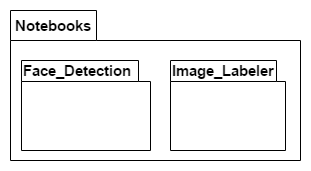
\includegraphics[width=0.4\textwidth]{dia_paquetes}
\caption{Diagrama de paquetes}
\label{fig:C.4.1}
\end{figure}

Por un lado, tenemos el módulo que se encarga de la gestión de carpetas donde el etiquetador almacena las imágenes. Véase el diagrama de clases \ref{fig:C.4.2}.

\begin{figure}[h]
\centering
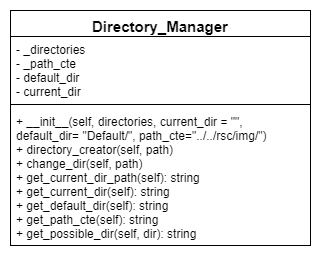
\includegraphics[width=0.7\textwidth]{dia_dirs}
\caption{Diagrama de clases de las clases encargadas de la gestión de carpetas}
\label{fig:C.4.2}
\end{figure}


Y, por otro lado, tenemos las clases encargadas de la predicción de una nueva imagen mediante el \textit{notebook} explicado anteriormente. En este caso existen 3 clases, las cuales interaccionan entre sí. La primera es una clase estática con 2 funciones para los cálculos del non-maximum suppression y la ventana deslizante. Véase la figura \ref{fig:C.4.3} 


\begin{figure}[h]
\centering
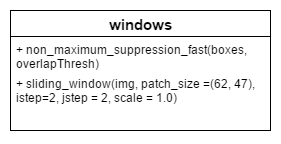
\includegraphics[width=0.4\textwidth]{dia_win}
\caption{Clase estática encargada de las tareas de non-maximum suppression y ventana deslizante}
\label{fig:C.4.3}
\end{figure}

Por otro lado, tenemos la clase encargada de envolver al clasificador y realizar las tareas de clasificación de una imagen. Véase la figura \ref{fig:C.4.4}.

\begin{figure}[h]
\centering
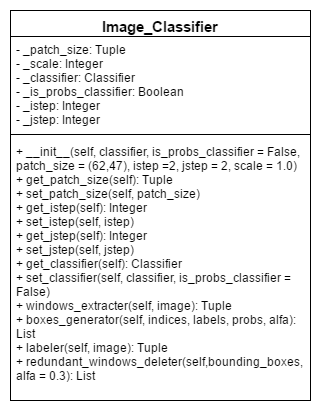
\includegraphics[width=0.4\textwidth]{dia_ic}
\caption{Clase encargada de las tareas de clasificación de una imagen}
\label{fig:C.4.4}
\end{figure}

Y, finalmente, tenemos la clase encargada de guardar la imagen, mostrarla y poder clasificarla con el apoyo del resto de clases. Véase la figura \ref{fig:C.4.5}.

\begin{figure}[h]
\centering
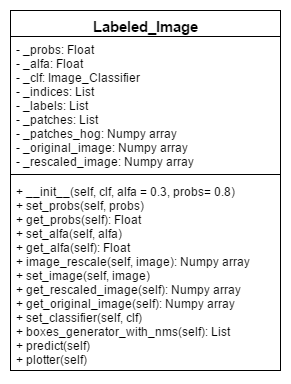
\includegraphics[width=0.4\textwidth]{dia_li}
\caption{Clase encargada de de guardar la imagen, mostrarla y poder clasificarla.}
\label{fig:C.4.5}
\end{figure}

Para finalizar esta sección, podemos apreciar en la figura \ref{fig:C.4.6} como interaccionan las tres clases.

\begin{figure}[h]
\centering

\includegraphics[width=0.99\textwidth]{dia_cls}
\caption{Diagrama de clases del \textit{Jupyter Notebook} para la detección de caras}
\label{fig:C.4.6}
\end{figure}

\section{Diseño de las interfaces}

En esta sección se explicarán las diferentes interfaces de los productos realizados en este trabajo fin de grado.

\subsection{\textit{Jupyter Notebook} para la detección de caras}

Durante el primer mes se trabajo en un \textit{Jupyter Notebook} que trataba de reconocer caras mediante un clasificador junto a un extractor de características, como ya hemos explicado en secciones anteriores. Con este \textit{Jupyter Notebook} se trataba de facilitar la evaluación del rendimiento de los clasificadores y el cambio de las distintas variables de manera interactiva. 

Por lo tanto, la interfaz de este \textit{Jupyter Notebook} no ha sido trabajada para su uso por parte del usuario. Sino que fue creada para un uso más de experimentación. Es por ello que la interfaz no tiene un buen grado de usabilidad como podemos observar en la figura \ref{fig:C.5.1}.

\begin{figure}[h]
\centering
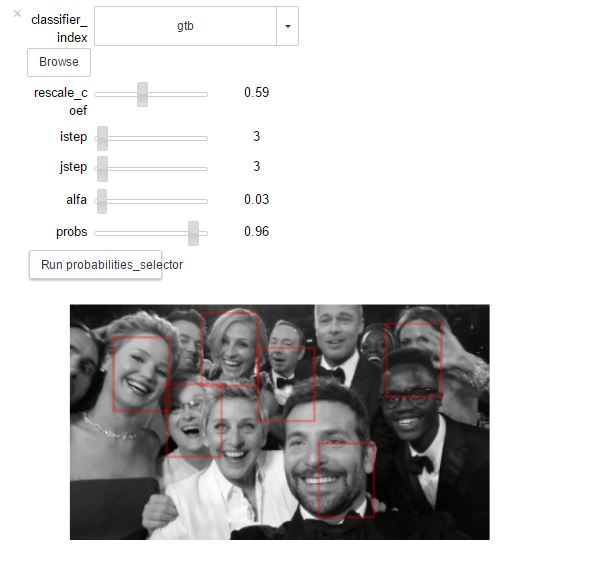
\includegraphics[width=0.99\textwidth]{reconocimiento_de_caras_notebook_v1}
\caption{\textit{Jupyter Notebook} para el reconomiento de caras}
\label{fig:C.5.1}
\end{figure}

Aun así, a continuación enumeraré y explicare la función de cada uno de los botones, o selectores de valores:

\begin{itemize}
	\item \textit{classifier_index}: permite seleccionar el clasificador con el que se desea clasificar la imagen.
	\item \textit{rescale_coef}: permite seleccionar el coeficiente de reescalado de una imagen.
	\item \textit{istep}: permite elegir el número de pixeles que debe saltar la ventana deslizante en cada subdivisión en el eje vertical.
	\item \textit{jstep}: permite elegir el número de pixeles que debe saltar la ventana deslizante en cada subdivisión en el eje horizontal.
	\item \textit{alfa}: permite seleccionar el coeficiente de solapación entre ventanas para que el método non-maximum suppression elimine más o menos ventanas solapadas.
	\item \textit{probs}: permite escoger las ventanas que deseamos mostrar en función de las probabilidades que indica el clasificador sobre cada ventana.
\end{itemize}

\subsection{Etiquetador de imágenes}

La interfaz del etiquetador de imágenes ha sido desarrollada partiendo del prototipo mostrado en la ilustración \ref{fig:C.5.2}. Tratando de crear una interfaz lo más simple e intuitiva para el usuario.

\begin{figure}[h]
\centering
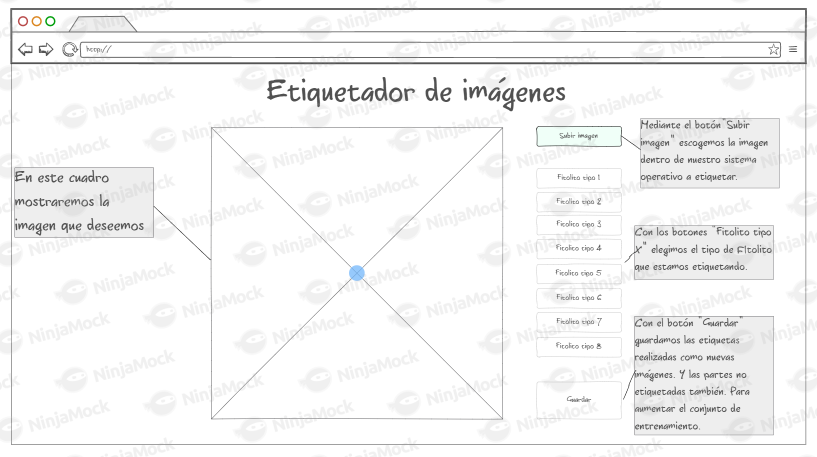
\includegraphics[width=0.99\textwidth]{protototipo_etiquetador_de_imagenes}
\caption{Prototipo del etiquetador de imágenes}
\label{fig:C.5.2}
\end{figure}

El resultado tras la implementación de este producto es el mostrado en la \ref{fig:C.5.3}. Obteniendo una interfaz muy similar a la prototipada en un principio. Pero añadiendo algún elemento más, para facilitar su uso por parte del usuario.

\begin{figure}[h]
\centering
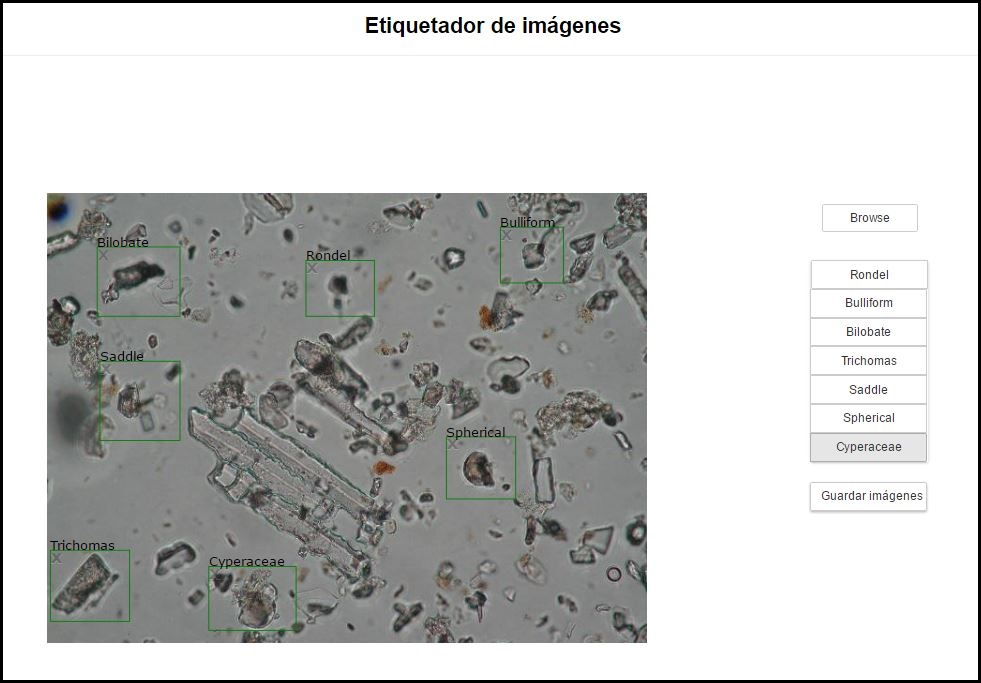
\includegraphics[width=0.99\textwidth]{etiquetador_de_imagenes_v1}
\caption{Etiquetador de imágenes}
\label{fig:C.5.3}
\end{figure}
\apendice{Documentación técnica de programación}

\section{Introducción}
En este anexo se introducirá todos los directorios, \textit{notebooks} y documentación útil necesaria para las personas que deseen continuar o trabajar en el proyecto.

\section{Estructura de directorios}
La estructura de directorios del proyecto, en estructura de árbol, es la siguiente:

\begin{itemize}
	\item \textit{\textbf{/}}, es decir, el directorio raíz. En el se encuentra el fichero de la licencia, el \textit{README}, el \textit{.gitignore} y las siguientes carpetas:
	\begin{itemize}
		\item \textit{\textbf{code}}: contiene toda la lógica de la aplicación.
			\begin{itemize}
				\item \textit{\textbf{imgaug}}: repositorio para realizar \textit{Data Augmentation} con \textit{Python 2}.
				\item \textit{\textbf{darkflow}}: repositorio para la detección de objetos en tiempo real.
				\item \textit{\textbf{notebooks}}: contiene todos los notebooks creados para este proyecto.
				\begin{itemize}
					\item Data\_Augmentation: contiene una serie de \textit{notebooks} para tareas de \textit{data augmentation}.
					\item Image\_Labeler: contiene el etiquetador de imágenes.
					\item Phytoliths\_Classifier: contiene varios \textit{notebooks} en los que se muestran ejemplos de clasificación y reconocimiento de fitolitos.
					\item Prototypes: contiene varios \textit{notebooks} prototipos.
				\end{itemize}
				\item \textit{\textbf{rsc}}: contiene los recursos necesarios por las distintas aplicaciones: imágenes y objetos. 
			\end{itemize}
		\item \textit{\textbf{doc}}: contiene la documentación del proyecto.
		\begin{itemize}
			\item \textbf{general\_doc}: contiene la memoria y los anexos del proyecto.
				\begin{itemize}
					\item \textit{\textbf{img}}: contiene todas las imágenes de la memoria y anexos del proyecto.
					\item \textit{\textbf{tex}}: contiene los ficheros correspondientes a cada uno de los anexos.
				\end{itemize}
			\item \textbf{source\_doc}: contiene la documentación del código.
			\item \textbf{test\_reports}: contiene los informes de cubrimiento del código.
		\end{itemize}
	\end{itemize}
\end{itemize}

\section{Manual del programador}

En este apartado se explican algunos aspectos sobre los dos \textit{notebooks} principales: etiquetador de imágenes y \textit{notebook} para el reconocimiento de fitolitos. Aunque sería aplicable a otros, como los desarrollados para realizar \textit{data augmentation}. 

\subsection{Etiquetador de imágenes}

En esta sección explicare más en detalle como funciona internamente el etiquetador.

\subsubsection{Base del etiquetador: \textit{Widgets} de \textit{ipywidgets}}

El etiquetador está creado mediante los \textit{Widgets} de \textit{ipywidgets} para \textit{Python}. Un \textit{Widget} es un objeto de Python con representación en navegadores. Este nos permite la comunicación entre \textit{JavaScript} y \textit{Python}. Facilitando, así, crear interfaces \textit{Web} interactivas, como es nuestro caso~\cite{ipywidgets:whataarewidgets}.

El etiquetador de imágenes es un \textit{Widget} personalizado, el cual ha sido creado por nosotros. Pero, además, este utiliza otros \textit{Widgets} prefedefinidos por los \textit{ipywidgets} para los botones.

\subsubsection{\textit{Javascript}}

La parte de código \textit{JavaScript} se ocupa de representar todos los elementos visuales y capturar los eventos.

En cuanto a elementos visuales, nos referimos al SVG, la imagen, rectangulos o etiquetas y textos. Los cuales son elementos \textit{HTML}. Y, en cuanto a eventos, nos referimos a los clicks o movimientos del ratón sobre nuestros elementos \textit{HTML}.

\subsubsection{\textit{Python}}

La parte de \textit{Python} controla toda la lógica de la aplicación. Desde que imagen se muestra, hasta las conversiones de las coordenadas de la imagen entre la vista y la imagen real.

Además, para los botones, los cuales son \textit{Widgets} de \textit{Python}, se controlan tambien sus eventos desde el propio \textit{Python}.

\subsection{Reconocimiento de fitolitos}

El \textit{notebook} para el reconocimiento de fitolitos ha sido creado basándonos en los \textit{widgets} predefinidos sobre los que en la sección anterior hablábamos. Por lo que la idea es similar a la anterior con la diferencia de que no se utiliza ningún \textit{widget} personalizado.

En cuanto al código que se encarga de detectar los fitolitos dentro de una imagen, este se encuentra documentado en la carpeta <<doc/general\_doc>> como previamente he indicado. En la figura~\ref{fig:D.3} muestro la portada de la documentación del código. Además, para tener una mayor compresión del código, se deben de consultar los anexos de diseño procedimental y los conceptos y aspectos relevantes de la memoria.

\begin{figure}
\centering
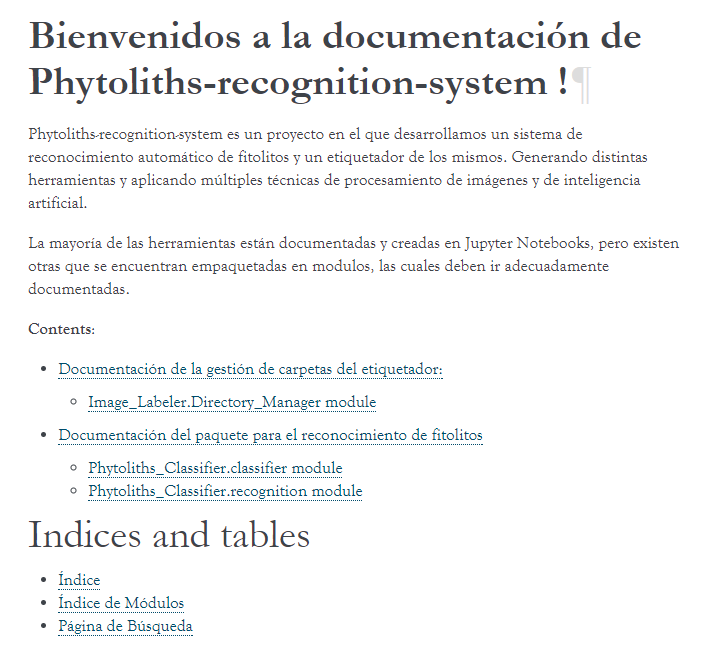
\includegraphics[width=0.99\textwidth]{docex}
\caption{Portada de la documentación del código}
\label{fig:D.3}
\end{figure}

\section{Compilación, instalación y ejecución del proyecto}

\subsection{Compilación, instalación y ejecución}

Los \textit{notebooks} llevan consigo la instalación de varias librerías, las cuales se indican en el \textit{Manual de uuario}. En ningún caso necesitan ser compilado, ni los \textit{notebooks} ni ningun fuente, al ser \textit{Python} un lenguaje interpretado.  

\subsection{Procedimiento de entrenamiento de \textit{YOLO}}

Para realizar el entrenamiento de \textit{YOLO}, \textit{darkflow} nos provee de un \textit{script} que nos facilita dicha tarea mediante la linea de comandos\footnote{Solo ha sido probado desde un sistema Linux.}, llamado \textit{flow}. Además, existen dos posibilidades principales para realizar el entrenamiento sobre nuestro \textit{dataset}:

\begin{itemize}
	\item Utilizar unos pesos\footnote{Pesos: son cada uno de los valores asignados a una neurona en una red neuronal.} pre-entrenados para nuestro modelo.
	\item Crear un modelo que se ajuste a nuestras necesidades.
\end{itemize}

La ventaja de utilizar unos pesos pre-entrenados reside en que la red neuronal ya habrá aprendido ciertas características, como bordes o formas. Por lo tanto, el tiempo de entrenamiento será mucho menor. Pero puede que la reutilización de dicho modelo no se adecue a nuestras necesidades ya sea porque tengamos un número distinto de clases al modelo inicial o porque el contexto sea totalmente distinto.

Por otro lado, se encuentra el entrenamiento desde cero de un nuevo modelo que se adecue a nuestras necesidades. El cual suple las desventajas presentadas por la anterior opción, pero introduce una mayor complejidad a la hora del entrenamiento.

En cualquier caso, los dos siguientes ejemplos, correspondientes a las opciones planteadas, nos permitirían entrenar el modelo:

\begin{verbatim}
flow --train --model cfg/yolo-tiny.cfg
 --load bin/yolo-tiny.weights
 --dataset "Fitolitos" --annotation "Fitolitos"

o

flow --model cfg/yolo-new.cfg --train
 --dataset "Fitolitos" --annotation "Fitolitos"
\end{verbatim}

Donde la opción \textit{--train} indica que se desea entrenar un modelo, la opción \textit{--load} indica donde se encuentran los pesos pre-entrenados, la opción \textit{--dataset} indica la ruta de la carpeta donde se encuentran las imagenes de los fitolitos y la opción \textit{--annotation} indica donde se encuentran los ficheros con las coordenadas\footnote{La modificaciones realizadas sobre \href{https://github.com/thtrieu/darkflow}{\textit{darkflow}} para permitir la lectura y conversión de mis coordenadas están pensados para que el valor de las opciones \textit{dataset} y \textit{annotation} sean el mismo. De otra manera el modelo fallará en el entrenamiento.}.

A modo de resumen, voy a enumerar todas las opciones que nos permite escoger la herramienta \textit{flow}:

\begin{itemize}
	\item \textit{imgdir}: ruta que contiene las imágenes con las que realizar pruebas.
	\item \textit{binary}: ruta que contiene los pesos.
	\item \textit{config}: ruta que contiene los ficheros de configuración.
	\item \textit{dataset}: ruta que contiene las imágenes.
	\item \textit{backup}: ruta que contiene las copias de seguridad de los pesos.
	\item \textit{summary}: ruta que contiene los resumenes \textit{TensorBoard}, los cuales se pueden abrir con una herramienta de \textit{TensorFlow}.
	\item \textit{annotation}: ruta que contiene los ficheros con las anotaciones o coordenadas de las etiquetas dentro de las imágenes.
	\item \textit{threshold}: umbral que determina las probabilidades mínimas que debe cumplir una detección o caja para mostrarse.
	\item \textit{model}: ruta al fichero de configuración deseado.
	\item \textit{trainer}: algoritmo de entrenamiento.
	\item \textit{momentum}: optimizador aplicable a los algoritmos de entrenamiento: \textit{rmsprop} y \textit{momentum}.
	\item \textit{verbalise}: mostrar como se forma el grafo o red neuronal.
	\item \textit{train}: entrenar la red neuronal.
	\item \textit{load}: inicialización de la red.
	\item \textit{savepb}: guardar configuración y pesos a un fichero \textit{protobuf}.
	\item \textit{gpu}: cantidad de la capacidad de los procesadores gráficos a utilizar.
	\item \textit{gpuName}: nombre de la tarjeta gráfica.
	\item \textit{lr}: tasa de aprendizaje para el entrenamiento.
	\item \textit{keep}: número de últimos resultados que se mantienen guardados.
	\item \textit{batch}: tamaño del lote de imágenes.
	\item \textit{epoch}: número de \textit{epochs}.
	\item \textit{save}: número de ejemplos tras los cuales se realiza una copia de seguridad.
	\item \textit{demo}: para realizar una demo con \textit{webcam}.
	\item \textit{queue}: tamaño del lote para la demo.
	\item \textit{json}: salida de las cajas en formato \textit{json}.
	\item \textit{saveVideo}: guardar video de la entrada de video o camara.
	\item \textit{pbLoad}: ruta del fichero \textit{protobuf}.
	\item \textit{metaLoad}: ruta del fichero .meta generado junto al fichero \textit{protobuf}.
\end{itemize}

\section{Pruebas del sistema}

En el desarrollo de cualquier sistema software es fundamental poseer una batería de teses con los cuales probar el correcto funcionamiento de nuestro sistema. En nuestro caso, desgraciadamente, el tiempo necesario para la investigación de las distintas técnicas y su aplicación nos ha dificultado en gran medida llevarlos a cabo con la perfección que nos hubiese gustado.

Sin embargo, hemos realizado varios teses unitarios, incluidos en <<code/tests>>, para las distintas clases que tenemos empaquetadas. En la figura~\ref{fig:D.1} se muestra un ejemplo. Además, bajo la carpeta <<doc/test\_reports>> hay varias carpetas con los informes de cubrimiento con el aspecto mostrado en la figura~\ref{fig:D.2}.

En cuanto a los \textit{Jupyter Notebooks}, sería interesante que en futuros desarrollos se utilizase un \textit{framework} para la automatización de teses de aplicaciones web como Selenium\footnote{\url{http://www.seleniumhq.org/}}.

\begin{figure}
\centering
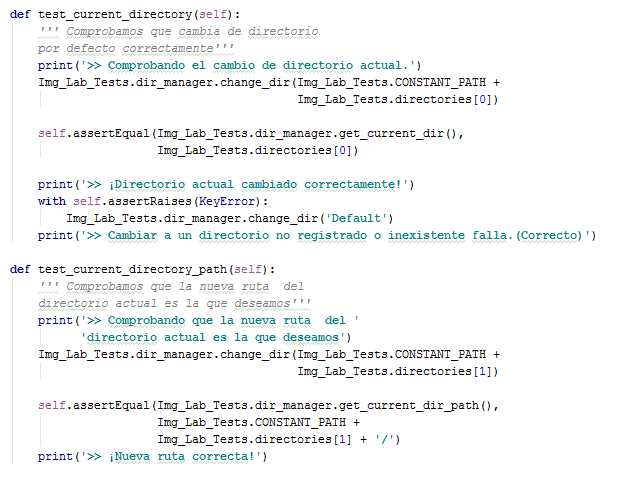
\includegraphics[width=0.99\textwidth]{testex}
\caption{Ejemplo de test unitario}
\label{fig:D.1}
\end{figure}

\begin{figure}
\centering
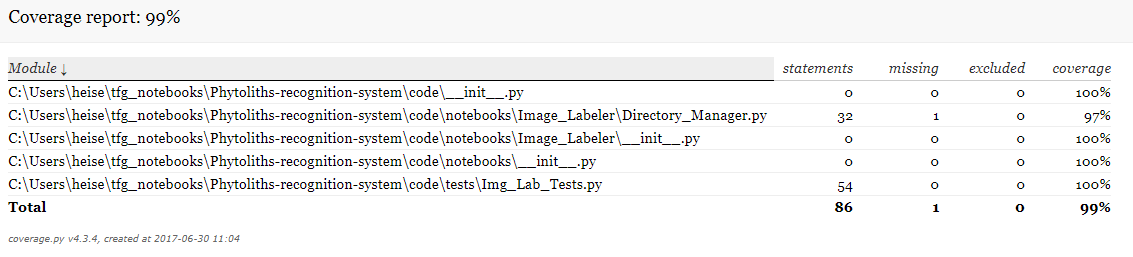
\includegraphics[width=0.99\textwidth]{covex}
\caption{Ejemplo de test unitario}
\label{fig:D.2}
\end{figure}
\apendice{Documentación de usuario}

\section{Introducción}

En esta sección se indicarán los distintos prerrequisitos de la herramienta. Así, como toda la información necesaria para la correcta utilización de la herramienta. O la solución ante posibles problemas en su utilización.

\section{Requisitos de usuarios}

El requisito básico necesario, por parte del usuario, es disponer de un ordenador con un sistema operativo moderno. Pudiendo, así, llevar a cabo la instalación que será explicada en la siguiente sección.

\section{Instalación}
Los requisitos necesarios son:

\begin{itemize}
	\item Anaconda\footnote{Es altamente recomendable utilizar \textit{Anaconda} para la instalación de \textit{Python} junto a algunos paquetes necesarios. Puesto que la instalación aislada de \textit{Python} llevaría al usuario a tener que instalar manualmente múltiples paquetes que ya vienen preinstálados con \textit{Anaconda}.}.

	\item IPython File Upload. Siguiendo los pasos de instalación en \url{https://github.com/peteut/ipython-file-upload}.

	\item \textit{Jupyter Dashboards}. Siguiendo los pasos de instalación en \url{https://github.com/jupyter/dashboards}.

	\item Este proyecto descargado o clonado. Cuyo enlace al repositorio es \url{https://github.com/jasag/Phytoliths-recognition-system}.
\end{itemize}

\section{Manual del usuario}

En esta sección se explicarán los distintos aspectos a tener en cuenta en el uso de los distintos productos.

\subsection{Manual del usuario: etiquetador de imágenes}

Una vez completados satisfactoriamente los pasos anteriores,  ejecutamos \textit{Jupyter Notebook} desde \textit{Anaconda}\footnote{ Si es la primera vez que utilizas Anaconda es recomendable utilizar Anaconda Navigator. Ya que este nos facilitará ejecutar \textit{Jupyter Notebook}, sin el uso de la linea comandos.}. Y desde esta aplicación, abrimos el \textit{notebook} \textit{Image\_Labeler.ipynb}, en la carpeta \textit{code/notebooks} dentro del repositorio previamente descargado.

Con \textit{Image\_Labeler.ipynb} ya abierto tendremos que llevar a cabo dos pasos:

\begin{enumerate}[1.]
    \item Ejecutar todas las celdas del \textit{notebook}.
    \item Activar \textit{Dashboard Preview}.
\end{enumerate}

Para llevar a cabo los dos siguientes pasos basta con navegar por la barra del \textit{notebook}, como muestro a continuación. 

Para la ejecución del primer paso, navegamos por \textit{Cell} y clicamos en \textit{Run All}. Como se puede observar en la figura \ref{fig:E.4.1}.

\begin{figure}[h]
\centering
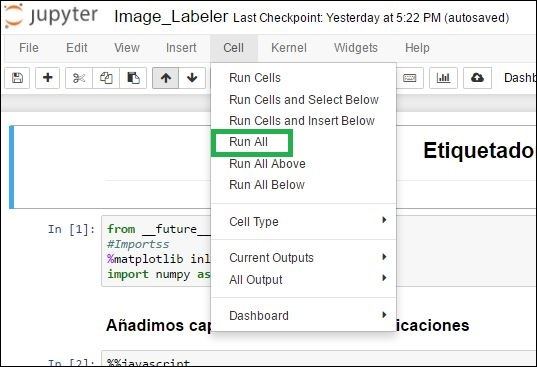
\includegraphics[width=0.80\textwidth]{ejecucion_todas_las_celdas}
\caption{Ejecución del \textit{notebook}}
\label{fig:E.4.1}
\end{figure}

Para la ejecución del segundo paso, navegamos por \textit{View} y clicamos en \textit{Dashboard Preview} \ref{fig:E.4.2}.

\begin{figure}[h]
\centering
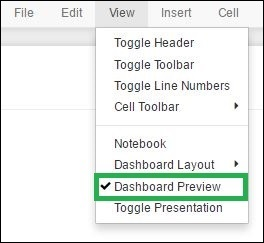
\includegraphics[width=0.60\textwidth]{cambio_de_vista_a_preview_dashboard}
\caption{Selección de la vista del \textit{notebook}}
\label{fig:E.4.2}
\end{figure}

Una vez realizados los pasos anteriores, tendremos como resultado la figura \ref{fig:E.4.3}.

\begin{figure}[h]
\centering
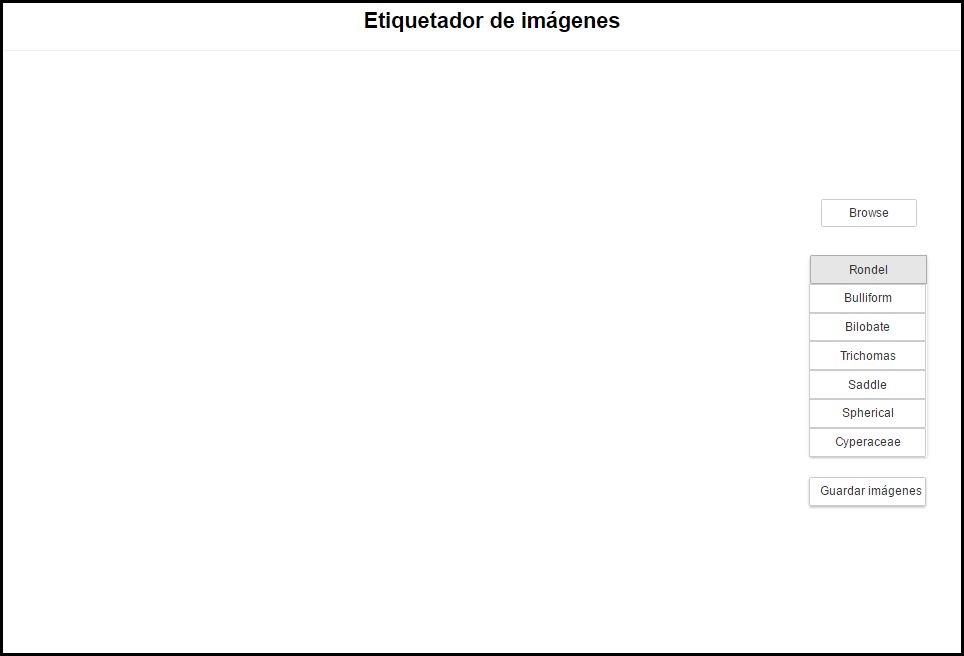
\includegraphics[width=0.99\textwidth]{etiquetador_de_imagenes_antes_de_cargar_imagen_v1}
\caption{Etiquetador de imágenes}
\label{fig:E.4.3}
\end{figure}

\subsubsection{Uso del etiquetador}

Como resultado de los pasos previos, el etiquetador de imágenes estará listo para su funcionamiento. 

El etiquetador está compuesto por dos partes principales:

\begin{itemize}
	\item Parte izquierda: imagen.
	\item Parte derecha: \textrm{<<botones>>}.	
\end{itemize}

La parte izquierda mostrará la imagen a ser etiquetada. Y la parte derecha mostrará los botones que nos permitirán realizar distintas elecciones. Como podemos ver en la figura \ref{fig:E.4.3}.

\subsubsection{Parte derecha del etiquetador}
La parte derecha del etiquetador esta compuesta por tres grupos de botones. El botón para la carga de una imagen, los botones de selección de fitolito y el botón de guardado. Como podemos obsevar en la figura \ref{fig:E.4.7}. 

En las secciones siguientes explicaré sus funciones. 

\begin{figure}[h]
\centering
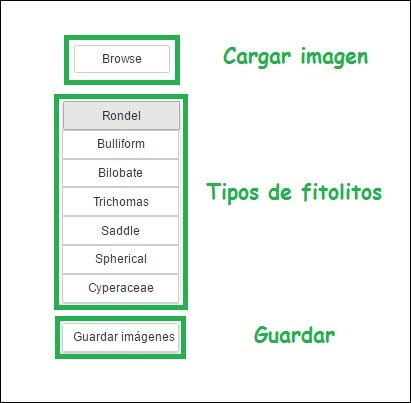
\includegraphics[width=0.50\textwidth]{etiquetador_botones}
\caption{Parte derecha del etiquetador}
\label{fig:E.4.7}
\end{figure}

\subsubsection{Carga de imagen}

Para etiquetar una imagen el primer paso será escoger una imagen en nuestro ordenador mediante el botón \textit{Browse}, situado en la esquina superior derecha del etiquetador. Como se puede ver en la figura \ref{fig:E.4.3}.

Una vez  pulsado, se mostrará una ventana, como la que podemos ver en la figura \ref{fig:E.4.4}, en la que escogeremos la imagen que deseemos.

\begin{figure}[h]
\centering
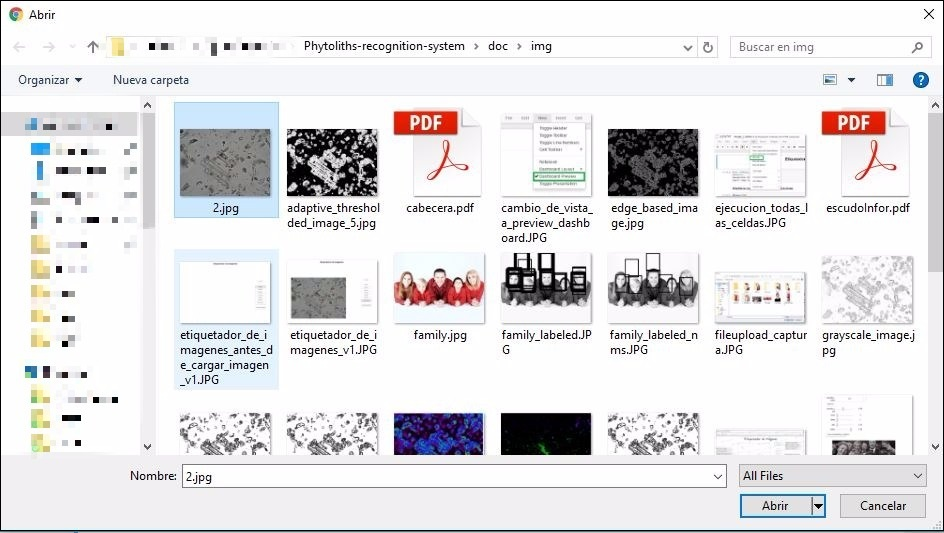
\includegraphics[width=0.99\textwidth]{fileupload_captura}
\caption{Ventana de subida de ficheros}
\label{fig:E.4.4}
\end{figure}

Tras escoger la imagen, esta se cargará en la parte izquierda del etiquetador, dando lugar a algo similar a lo mostrado en la figura \ref{fig:E.4.5}.

\begin{figure}[h]
\centering
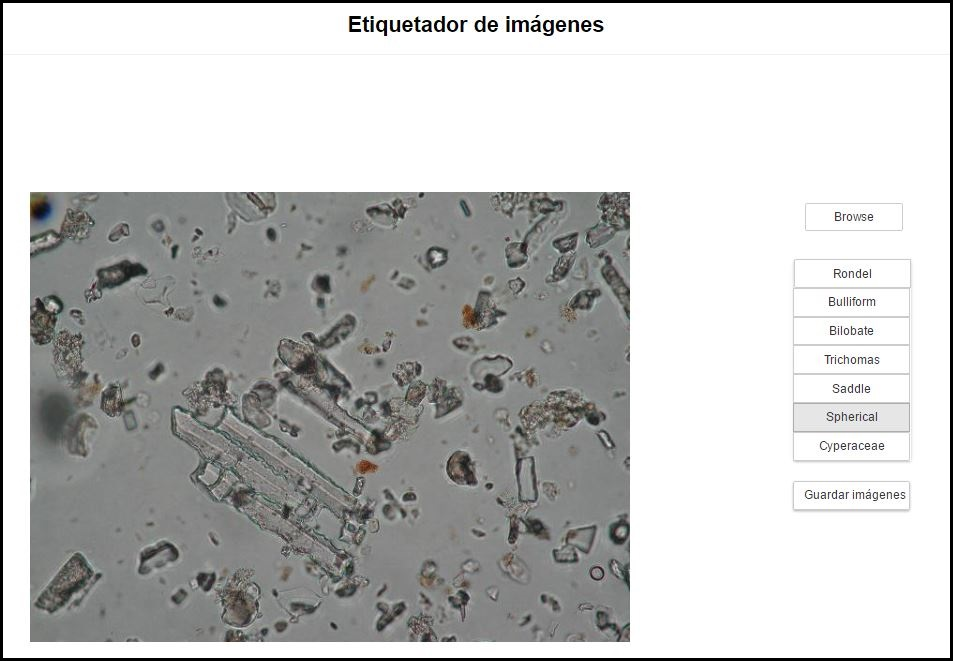
\includegraphics[width=0.99\textwidth]{etiquetador_de_imagenes_2_v1}
\caption{Etiquetador imágenes con una imagen cargada}
\label{fig:E.4.5}
\end{figure}

\subsubsection{Etiquetar distintos tipos de fitolitos}
Antes de explicar como se crean las etiquetas, debemos de tener en cuenta los botones para la selección de tipos de fitolito.

Cada vez que se quiera etiquetar un tipo de fitolito distinto tendremos que clicar en el botón correspondiente al tipo de fitolito objetivo.

A su vez, y para facilitarnos distinguir a que tipo de fitolito pertenece cada etiqueta, se escribe encima de cada etiqueta el tipo de fitolito que ha sido etiquetado, como podemos ver en la figura \ref{fig:E.4.6}.

\begin{figure}[h]
\centering
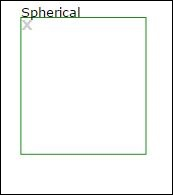
\includegraphics[width=0.30\textwidth]{etiqueta_ejemplo}
\caption{Ejemplo de etiqueta}
\label{fig:E.4.6}
\end{figure}

\subsubsection{Realizar etiquetas}

Una vez cargada la imagen en el etiquetador y comprendido el uso de los botones de selección de tipo de fitolito, podemos comenzar a  etiquetar fitolitos. Para etiquetar basta con clicar en la imagen, mover el ratón hacía donde deseemos y volver a clicar. Para, así, definir una etiqueta como la que se puede ver en la figura \ref{fig:E.4.6}.

\subsubsection{Eliminar etiquetas}

Como es normal, un usuario puede equivocarse realizando una etiqueta que no debería. Por ello, en la esquina superior izquierda de cada etiqueta, disponemos de una \textrm{<<X>>}, como podemos observar en la figura \ref{fig:E.4.6}, que nos permitirá eliminar etiquetas previamente realizadas. Posibilitando así revertir un error del usuario.

\subsubsection{Guardar etiquetas}
Después de realizar las etiquetas, y finalizar de etiquetar una imagen, solo queda guardar las etiquetas. Para ello basta con clicar el botón \textrm{<<Guardar imágenes>>} en la esquina inferior derecha del etiquetador, véase \ref{fig:E.4.3}.

Es \textbf{importante} destacar que no sirve de nada etiquetar una imagen, sino pulsamos más tarde en el botón guardar. Debido a que las etiquetas realizadas no habrán sido guardadas. Y 
, por lo tanto, todas las etiquetas realizadas sobre una imagen se perderán.

\subsubsection{Etiquetas realizadas fuera de la imagen}

En la versión actual del etiquetador, este te permite realizar etiquetas fuera de la imagen. Pero estas etiquetas no serán guardadas.

Por lo tanto, debemos de tener en cuenta que las etiquetas que no tengan todas sus aristas dentro de la imagen no se guardan.

Aun, así, en la siguiente sección explicaré como comprobar que las etiquetas previamente realizadas han sido guardadas.

\subsubsection{Carga de etiquetas previamente realizadas}

Las imágenes etiquetadas se guardan en la carpeta \textit{/code/rsc/img} dentro del repositorio. Al cargar imágenes que se encuentren dentro de esta carpeta, las etiquetas previamente realizadas sobre estas imágenes se cargarán con ellas\footnote{Notese que los nombres de las imágenes no son los cargados originalmente, ya que todas las imágenes etiquetadas son renombradas para no sobrescribir imágenes previamente etiquetadas con nombres iguales.}. Pudiendo ser modificadas, eliminándolas o creando nuevas etiquetas.

\subsubsection{Notificaciones}

Se han incluido en el etiquetador una sería de notificaciones, las cuales nos permitirán cercionarnos de distintos eventos. 

Las notificaciones que se muestran son las siguientes:

\begin{enumerate}
	\item Notificación en la carga de una imagen. Véase la figura \ref{fig:E.4.8.1}.
	\item Notificación en la carga incorrecta de un fichero que no sea una imagen. Véase la figura \ref{fig:E.4.8.2}.
	\item Notificación en el guardado de etiquetas. Véase la figura \ref{fig:E.4.8.3}.
\end{enumerate}

Gracias a estas notificaciones podremos saber si la imagen que hemos seleccionado era correcta, o no, y si las etiquetas ya han sido guardadas.

\begin{figure}[h]
\centering

\includegraphics[width=0.60\textwidth]{notificacion_carga_de_imagen_correctamente}
\caption{Notificación en la carga de una imagen}
\label{fig:E.4.8.1}
\end{figure}

\begin{figure}[h]
\centering

\includegraphics[width=0.70\textwidth]{notificacion_carga_de_imagen_incorrectamente}
\caption{Notificación en la carga incorrecta de un fichero que no sea una imagen}
\label{fig:E.4.8.2}
\end{figure}

\begin{figure}[h]
\centering

\includegraphics[width=0.70\textwidth]{notificacion_guardado_correctamente}
\caption{Notificación en el guardado de etiquetas}
\label{fig:E.4.8.3}
\end{figure}

\subsubsection{Bloqueo del etiquetador}

En algunas ocasiones, y por razones que desconozco hasta el momento, el etiquetador puede bloquearse alguna vez al cargar imágenes previamente etiquetadas. Para solucionar este problema basta con recargar el etiquetador, como se vio en la parte inicial de esta sección.


\bibliographystyle{plain}
\bibliography{bibliografiaAnexos}

\end{document}
